% Skrivet av Hariz Hasecic till Yrkeshögskolan Newton
% 2019
% Detta dokument ska tjäna som en mall för framtida examensarbeten, projektrapporter och övrigt redovisningsmaterial som kan tänkas förekomma. 
%Denna notis får ej tas bort.


%%%%%%%%%%%%%%%%%%%%%%%%%%%%%%%%%%%%%%%%%%%%%%%%%
%%%%%%%%%%%%%%%%%%%%%%%%%%%%%%%%%%%%%%%%%%%%%%%%%
\documentclass{article}
\usepackage{makeidx}            %För att skapa index i slutet
\makeindex

\usepackage[utf8]{inputenc}     % for éô
\usepackage[swedish]{babel}     % ord ska brytas korrekt på radslut
\usepackage[T1]{fontenc}        % for åäö
\usepackage[a4paper, left=1.5in, right=1.5in, top=1.5in, bottom=1.5in]{geometry}
                                % for page size and margin settings
\usepackage{graphicx}           %  
\usepackage{subcaption}         % För captions under bilder
\usepackage{wallpaper}          % För stor bild i titelsidan - BEHÖVS NOG INTE
\usepackage{eso-pic} %För mer wallpaper skit


\usepackage{eso-pic}            %för genomskinliga bilder med \/
\usepackage{transparent}        %för genomskinliga bilder (den på titelsidan)

\usepackage{amsmath,amssymb}    % 
\usepackage{amsthm}             % Vid behov av matte formler
\usepackage{mathtools}          % 
\usepackage{enumitem}           % för listor

\usepackage{lastpage}           %För att visa sista sidan på footer

\usepackage{listings}           % for control of 'itemize' spacing
\usepackage{todonotes}          % Gör TODO anteckningar
\usepackage{hyperref}           % sidhänvisningar och refs blir klickbara

\usepackage{etoolbox}           % För ifsatser,listor, etc

\usepackage [autostyle, english = american]{csquotes}
\MakeOuterQuote{"}

\usepackage{ifthen} % denna också för if satser
\usepackage{pgffor}             % för forloopar
\usepackage{fancyhdr}           % för headers/footers
\pagestyle{fancy}
\fancyhf{}


 

%%% Dokumentlogik- RÖR EJ %%%%%%%%%%%%%% RÖR EJ %%%%%%%%%%%%%%%
%%%%%%%%%%%%%%%%   RÖR EJ %%%%%%%%%%%%%% RÖR EJ %%%%%%%%%%%%%%%
%%%%%%%%%%%%%%%%%%%%%%%%%%%%%%%%%%%%%%%%%%%%%%%%%%%%%%%%%%%%%%%
%%%%%%%% Översätter några LaTex Kommandon. %%%%%%%%%%%%%%%%%%%% 
% Vill du använda andra kommandon så kanske dom är på engelska.
%                                                             %
%                                                             %
%                                                             %
%% För PDF METADATA                                           %
\title{\projekttitel}                                         %
\author{\forfattareett\space\forfattaretvo}                   %
\date{\projektdatum}                                          %
%                                                             %
\newcommand{\citat}[1]{\cite{#1}}                             %
\theoremstyle{remark}                                         %
\newtheorem*{remark}{Anmärkning}                              %
\newenvironment{anmarkning}[1]                                %
    {\begin{remark}{#1}}                                      %
    {\end{remark}}                                            %
\let\undersektion\subsection                                  %
\let\nysida\newpage                                           %
\let\nummerlista\enumerate                                    %

%Konstig när man översätter- Lämnar sista punkt icke-identerad.
\let\lista\itemize                                            %
\let\sak\item                                                 %
                                                              %

\let\hogerhuvud\rhead                                         %
\let\vansterhuvud\lhead                                       %
\let\hogerfot\rfoot                                           %
\let\sidan\thepage                                            %
\let\sektion\section                                          %
\let\undersektion\subsection                                  %
%% TODO PAket för snabba mini-anteckningar.    %%%%%%%%%%%%%%&          
\newcommand{\attskriva}[1]{\todo[inline,color=yellow!10]{ATT SKRIVA: #1}}

\newcommand{\kommentar}[1]{\todo{#1}}
%%%%%%%%%%%%%%%%%%%%%%%%%%%%%%%%%%%%%%%%%%%%%%%%%%%%%%%%%%%%%%%
%%%%%%%%%%%%%%%%%%%%%%%%%%%%%%%%%%%%%%%%%%%%%%%%%%%%%%%%%%%%%%%
\newcounter{Authorcount}                                      %
\newcounter{Supervisorcount}                                  %
\newcounter{Consultantcount}                                  %
\newcounter{Orgcount}                                         %
                                                              %
%Appendar forfattare still ny lista authors                   %
\newcommand{\nyforfattare}[1]                                 %
{\listcsgadd{Authors}{#1}\stepcounter{Authorcount}}           %
\newcommand{\nyhandledare}[1]                                 %
{\listcsgadd{Supervisors}{#1}\stepcounter{Supervisorcount}}   %
\newcommand{\nykonsult}[1]                                    %
{\listcsgadd{Consultants}{#1}\stepcounter{Consultantcount}}   %
\newcommand{\organisation}[1]                                 %
{\listcsgadd{Organizations}{#1}\stepcounter{Orgcount}}        %
                                                              %
\newcommand{\visalista}[2]      %Printar lista                %
{                                                             %
    \emph{#1}                                                 %
    \renewcommand{\do}[1]{\item[##1] \csuse{##1} \vskip-1mm}  %
    \dolistcsloop{#2}                                         %
     ~\\ ~\\                                                  %
}                                                             %
%%%%%%%%%%%%%%%%%%%%%%%%%%%%%%%%%%%%%%%%%%%%%%%%%%%%%%%%%%%%%%%

%%%%%%%%%%%%%%%%%%%%%%%%%%%%%%%%
%%   Byt titelvärden här      %%
%%%%%%%%%%%%%%%%%%%%%%%%%%%%%%%%
%             ||               %
%             ||               %
%             \/               %
\def\projekttitel{Rapport över Projektarbetet}
\def\undertitel{ObjektOrienterad Grundkurs HT2019}

\nyforfattare{Hariz Hasecic}

%
\nyhandledare{Aysen Furhoff}
\nyhandledare{Jesse Korinth}
\nyhandledare{Emelie Gruséus}

%
%Inga konsulter               
%                              %
%                              %
%%%%%%%%%%%%%%%%%%%%%%%%%%%%%%%%
%
%Lägg till grejer här på TITELSIDAN HÄR NEDAN
%||||||||||||||||||||||||||||||||||
%             ||
%             \/


\def\projektdatum{\today}

\hogerfot{\today}
\lfoot{\sidan}
\hogerhuvud{Rapport över Projektarbete}
\vansterhuvud{Grupp 1}
%             /\               %
%             ||               %
%             ||               %
%%%%%%%%%%%%%%%%%%%%%%%%%%%%%%%%
%%    Byt Titel värden här    %%
%%%%%%%%%%%%%%%%%%%%%%%%%%%%%%%%

\newcommand\BackgroundPic{%
\put(0,-510){%
\parbox[b][\paperheight]{\paperwidth}{%
\vfill
\centering
{\transparent{0.4}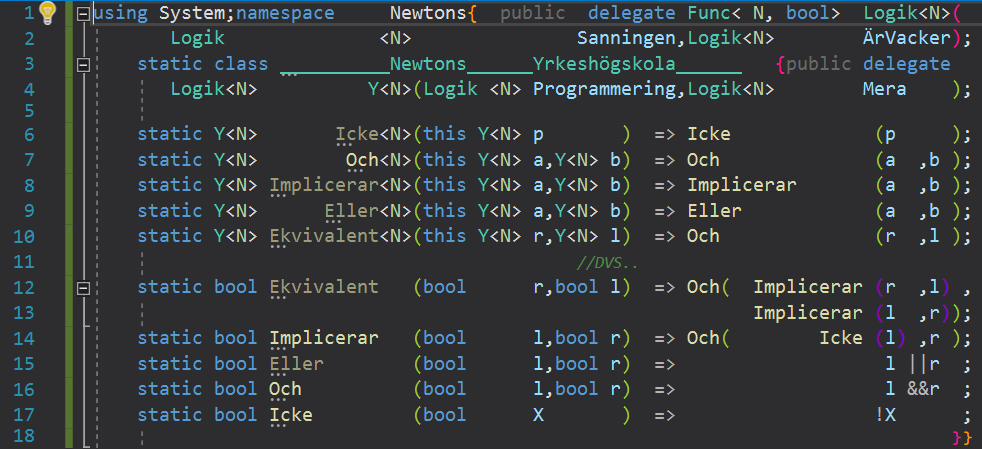
\includegraphics[width=\paperwidth,height=\paperheight,%
keepaspectratio]{img/GreatCodePredicates_small.PNG}}%
\vfill
}}}

\begin{document}
\begin{titlepage}
	\thispagestyle{empty}
	\newcommand{\HRule}{\rule{\linewidth}{0.5mm}}
	\center
	\textsc{\Large Newton Yrkeshögskola}\\[.7cm]
	
\includegraphics[width=25mm]{img/NewtonLogo.png}\\[.5cm]
	\textsc{Data Sektionen}\\[0.5cm]
	\HRule \\[0.6cm]
	{ \huge \bfseries \projekttitel}\\[0.1cm]
	\textsc{\undertitel}\\
	\HRule \\[.7cm]
	\textsc{\large .Net Systemutveckling}\\[.5cm]
	\begin{minipage}[t]{0.4\textwidth}
	\begin{flushleft}\large
    
%%%%%%%%%%%%%%%%%%%%%%%%%%%%%%%%%%%%%%%%%%%%%%%%%%%%%%%%%
%%%%%%%%%%%%%%%%% RÖR INGET I BOXEN NEDAN %%%%%%%%%%%%%%%
%                                                      %%
%                                                       %
    \newcommand{\testauthorcount}                       %
        {\ifthenelse{                                   %
        0< \arabic{Authorcount}                         %
        }                                               %
            {\visalista{Författare}{Authors}}           %
            {}                                          %
        }                                               %
    \testauthorcount                                    %
                                                        %
	\end{flushleft}                                     %
	\end{minipage}                                      %
	~                                                   %
	\begin{minipage}[t]{0.4\textwidth}                  %
	\begin{flushright} \large                           %
                                                        %
    \newcommand{\testsupervisorcount}                   %
        {\ifthenelse{                                   %
        0< \arabic{Supervisorcount}                     %
        }                                               %
            {\visalista{Handledare}{Supervisors}}       %
            {}                                          %
        }                                               %
    \testsupervisorcount                                %
                                                        %
    \newcommand{\testConsultantcount}                   %
        {\ifthenelse{                                   %
        0< \arabic{Consultantcount}                     %
        }                                               %
            {\visalista{Konsulter}{Consultants}}        %
            {}                                          %
        }                                               %
    \testConsultantcount                                %
                                                        %
	\newcommand{\testorgcount}                          %
        {\ifthenelse{                                   %
        0< \arabic{Orgcount}                            %
        }                                               %
            {\visalista{Företag}{Organizations}}        %
            {}                                          %                                                              %
        }                                               %      
    \testorgcount                                       %
	\end{flushright}                                    % 
	\end{minipage}\\[1cm]                               %
 	%\vfill                                              %
%	{\large \projektdatum}\\        

	

	\clearpage                                          %
\end{titlepage}                                         %
\AddToShipoutPicture{\BackgroundPic}

%                                                       %
%                                                       %
%%%%%%%%%%%%%%%%%%%%%%%%%%%%%%%%%%%%%%%%%%%%%%%%%%%%%%%%%  


	
\newpage
\sektion*{Abstrakt}
Detta är en rapport för ett projektarbete på sex personer på yrkeshögskolan Newton. Projektarbetet är för kursen "Objektorienterad programmering - Grundkurs" under Höstterminen 2019 och är lämpad att sammanfatta alla processer i framställningen av projektet. Implementerades sker med C\#. Dock kommer källkoden för projektet ej redovisas i just denna rapport utan endast arbets- och relationsprocesserna. Det inkluderas även enklare feedback till kursen samt några avslutande kommentarer kring projektets framgång. För källkod se: \url{https://github.com/AdaptiveStep/PizzaPalatsetG1}

\newpage
\tableofcontents                              
\newpage

\section*{Introduktion}
Projektet gick ut på att lärarna skulle anta rollen som "Beställare och Kravställare" samtidigt som eleverna antar rollen som "Leverantörer och Systemutvecklare". Vi bestämde oss att göra plan enligt följande.
\index{Roller!Leverantörer}
\index{Roller!Kravställare}
\index{Roller!Systemutvecklare}
\index{Roller!Beställare}

\paragraph{Milstolpar}
Det fanns ett par milstolpar som gruppen antog i början av projektet. Bland dessa ingick förutom kursplanens uppenbara examinationsmoment\footnote{Redovisning och produktion av \index{Milstolpar}Balsamiq Mockup, UML Diagram samt implementation med C\# kod} följande milstolpar som gruppen själv satte som delmål:\footnote{Vi använder begreppen Etapp och Milstolpe synonymt.}
\begin{itemize} 
    \item Etapp1: Förarbete 
    \item Etapp2: Huvudarbete/huvudfasen
    \item Etapp3: Avslutningsarbetet
\end{itemize}
Förutom dessa inkluderade vi förstås även mindre partiella delmål som kommer diskuteras senare i rapporten. Följande sektioner kommer nu i huvudsak men kortfattat redovisa dessa tre etapper.

\sektion{Förarbetet}
I denna process ingick både planeringsfas av arbetsprocessen samt initiering av gruppens användning av Google Drive. Det tog inte länge innan hela uppsättningen för vår "synkroniserade filhantering" kunde användas. Vi ansåg att en gemensam plattform för projektrelaterad fildelning var så viktig att det behövde göras före allt annat. Dock sköt vi upp GIT-hanteringen planerna kring dess användning för senare skeden. I förarbetet ingick även en  \index{Rollfördelning}rollfördelning av följande roller\footnote{Denna rollfördelning var preliminär, ej bindande utan fungerade endast förslag och vägledning} (vilka även detaljeras något i Figur \ref{fig:roller} på sida \pageref{fig:roller}): 

\begin{itemize}
    \item Arbetsledare
    \item Sekreterare
    \item DevOpsledare
    \item Designgruppen (två personer)
    \item Redovisningsledare
\end{itemize}
\begin{figure}
    \vspace{-2cm}
    \begin{subfigure}[b]{\textwidth}
        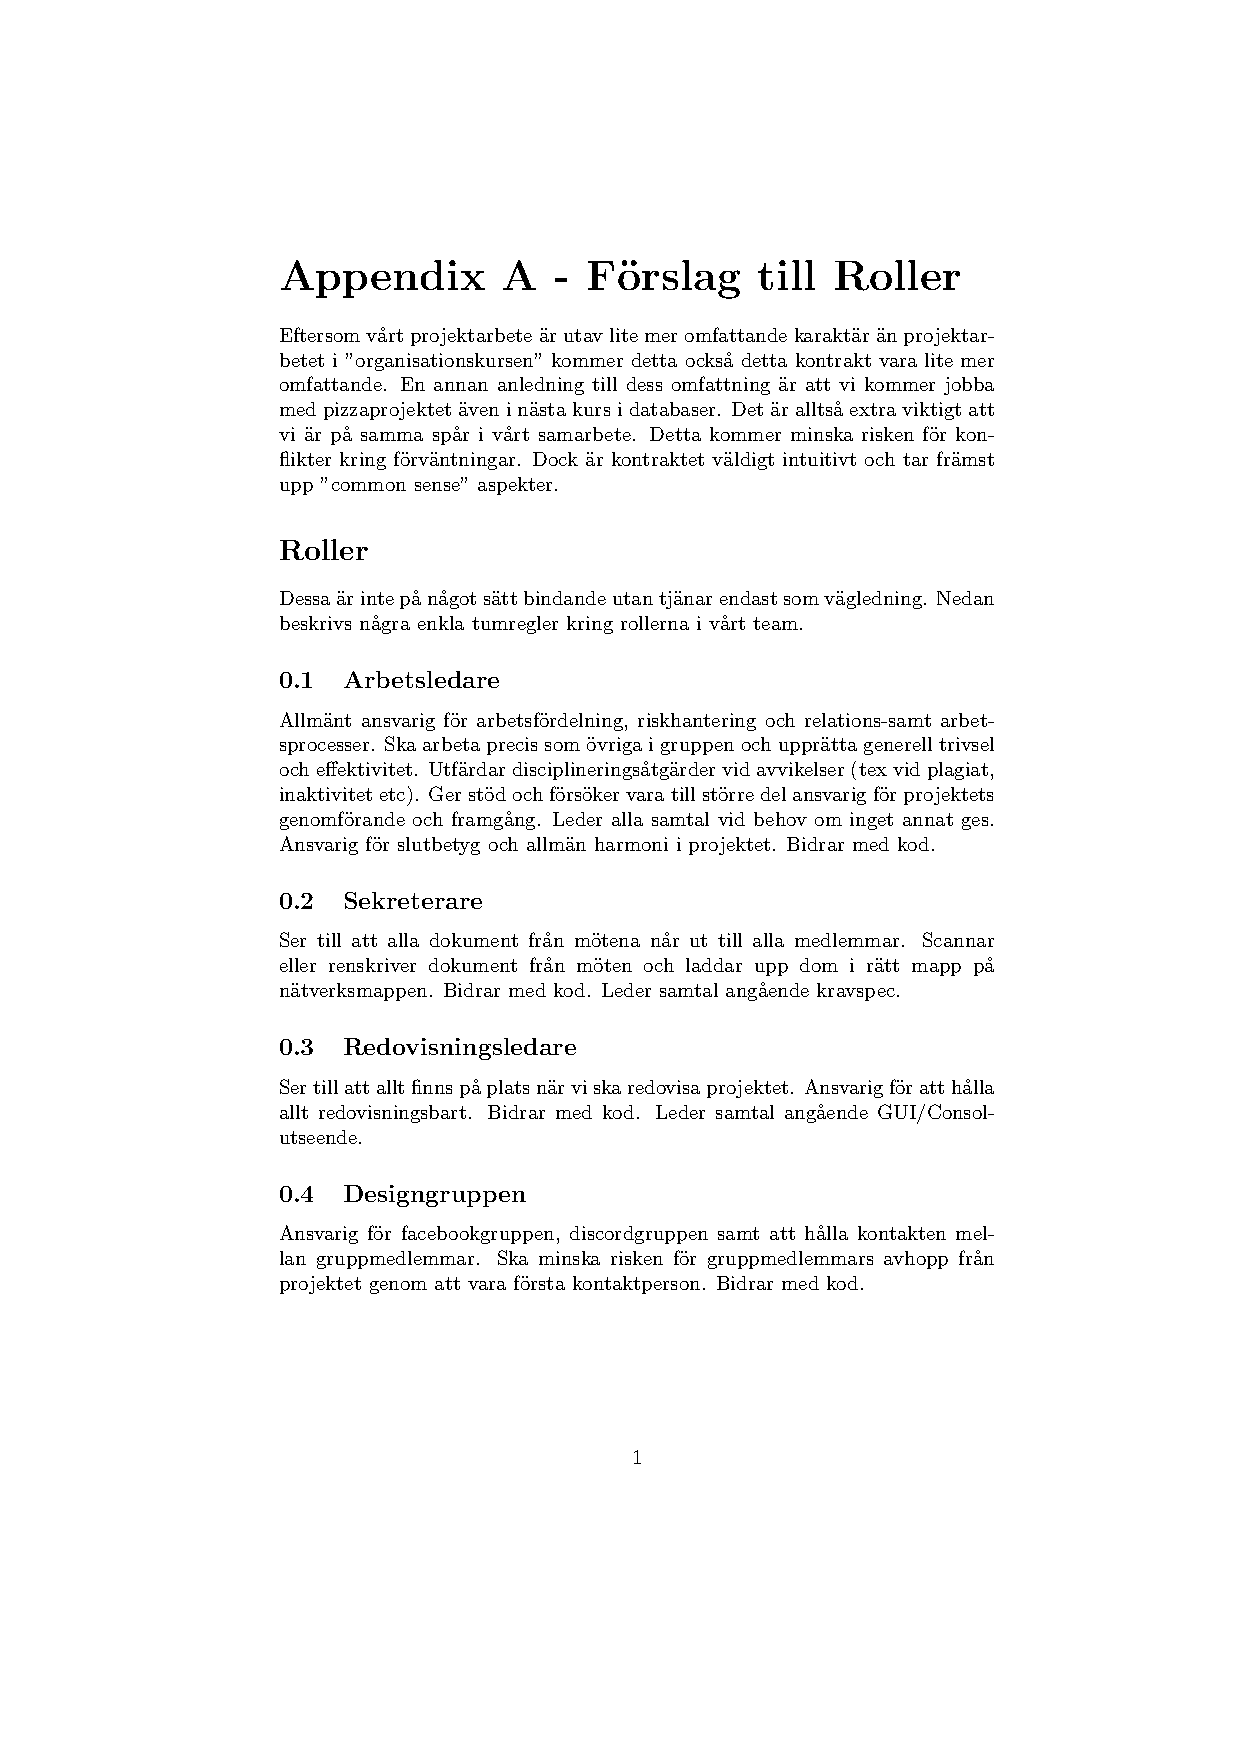
\includegraphics[width=\textwidth]{img/Appendix_A___Roller.pdf}
        \vspace{-5cm}
        \caption{Detaljer kring några av rollerna som delades ut till gruppen}
        \label{fig:roller}
    \end{subfigure}
     \vspace{1cm}

    ~
    \begin{subfigure}[b]{\textwidth}
        
\includegraphics[width=\textwidth]{img/Skissbilder/KundTerminalLogo.PNG}
        \caption{Screenshot av Kundterminalen}
        \label{fig:kundterminal}
    \end{subfigure}
    \caption{Några inblickar över det som producerades under projektet.}
    \vspace{5cm}

\end{figure}

\subsection{Tekniska problem och initial gruppdynamik}
Några tekniska problem som vi stötte på var bland annat att bestämma plattform för fildelningen dåd några av medlemmarnas initiala installation inte kunde synkronisera filer konsekvent.
Även \index{GIT!Github} Github deployment fick vänta tills nästa etapp i arbetsprocessen då endast en av medlemmarna hade erfarenhet med denna teknik. Dock ordnade sig allt i slutändan med undantaget att allt fick \index{GIT!Commit} comittas till masterbranch direkt, vilket naturligtvis var suboptimalt då risken fanns för destabiliserande \index{GIT!Push}pushningar. Gruppen accepterade denna risk samt att vår repository \index{GIT!Repository} var offentlig. Förarbetet medförde flera överenskommelser om regelbundna möten, dels pågrund av dessa tekniska problem dels på grund utav behovet av direkt kommunikation. Klockan 10:00 varje onsdag hade vi dessa då lektioner inte förekom på onsdagar. Ett gruppdynamiskt problem var då förstås att antalet deltagare vid varje möte kunde bli relativt oregelbundet. När väl alla synkade mappar låg uppe, gruppkontrakt hade skrivits på och konsensus kring arbetsprocess hade etablerats kände vi oss redo att ta projektet till nästa etapp. Dock skulle vi ha en öppen dialog kring planerna på rullande band vilket innebar att en viss flexibilitet av planerna ändå fanns där.

Utöver det övergripande förarbetet runt hela projektet fanns det även mindre etapper inför varje uppgift. Nästa sektion kommer beskriva hur vi hanterade detta m.h.a våra "Roadmaps". Slutligen kan tillägas att respekt för varandras förkunskaper, erfarenhet samt variansen av dessa genomsyrade hela projektets arbets-och relationsprocess. Ty, endast kunskaper som "hittills" ackumulerades från kursplanen skulle kunna förväntas från gruppens samtliga medlemmar. I början förekom ett visst missförstånd kring denna regel då förslag till olika lösningar inte alltid föreföll konsekvent med vår "Förkunskapsregel"\footnote{Om vi får kalla det så.}. Som exempel på min egna överträdelse för denna regel föreslog jag personligen ett sökträd som datastruktur för menysystemet. Detta skulle vara en lämplig lösning i allmänna fall men inte för omständigheterna kring gruppens "Förkunskapsregel". Även andra olämpligt komplicerade förslag gavs från andra medlemmar men detaljerna kring dessa är irrelevanta för rapportens ändamål. Ett exempel på hur ett av våra terminaler blev i slutändan kan ses i Figur \ref{fig:kundterminal}.

\section{Huvudarbetet}
Denna etapp var den som överlägset tog upp mest tid i både möten, inlärning (av UML), förberedelser och mer. Precis som i förarbetet hade vi regelbundna möten samt regelbunden kontakt via FaceBook Messenger, Discord\footnote{ett chatprogram för gruppchat med röst} och Gmail (dock inte via GitHub). Med vårt gruppkontrakt och vår öppna dialog flöt arbetet på exceptionellt bra. En av överenskommelserna som jag personligen fann utav anmärkningsvärd betydelse var att \emph{inga nya medlemmar skulle tillkomma} utan att gruppen röstat om det. Anledningen till detta är att det föregående projektet i denna utbildning\footnote{Entreprenörskap och organisation Grundkurs HT2019} gav oss nya medlemmar på rullande band och som konsekvens tvingade oss att börja om stora delar av relationsprocessen på nytt kring projektet. Detta olämpliga inflöde av nya medlemmar förde (utöver den orättvisa fördelningen av arbetet) även ett överskott av medlemmar vilket gjorde gruppen för stor.

Konsensus i gruppen har aldrig varit ett problem för oss i Grupp1 och en stor del av denna samverkan skulle kunna förklaras av ett gott förarbete. Våra "Roadmaps" såg ut enligt tabell \ref{fig:Roadmaps} på sidan \pageref{fig:Roadmaps}. Här går att se hur projektet och roadmapen utvecklades över tiden. Från denna får man även en liten inblick över hur arbetsbördan ökade för varje roadmap.

\begin{figure}
    \index{Roadmaps}
    \centering
    \begin{subfigure}[b]{0.3\textwidth}
        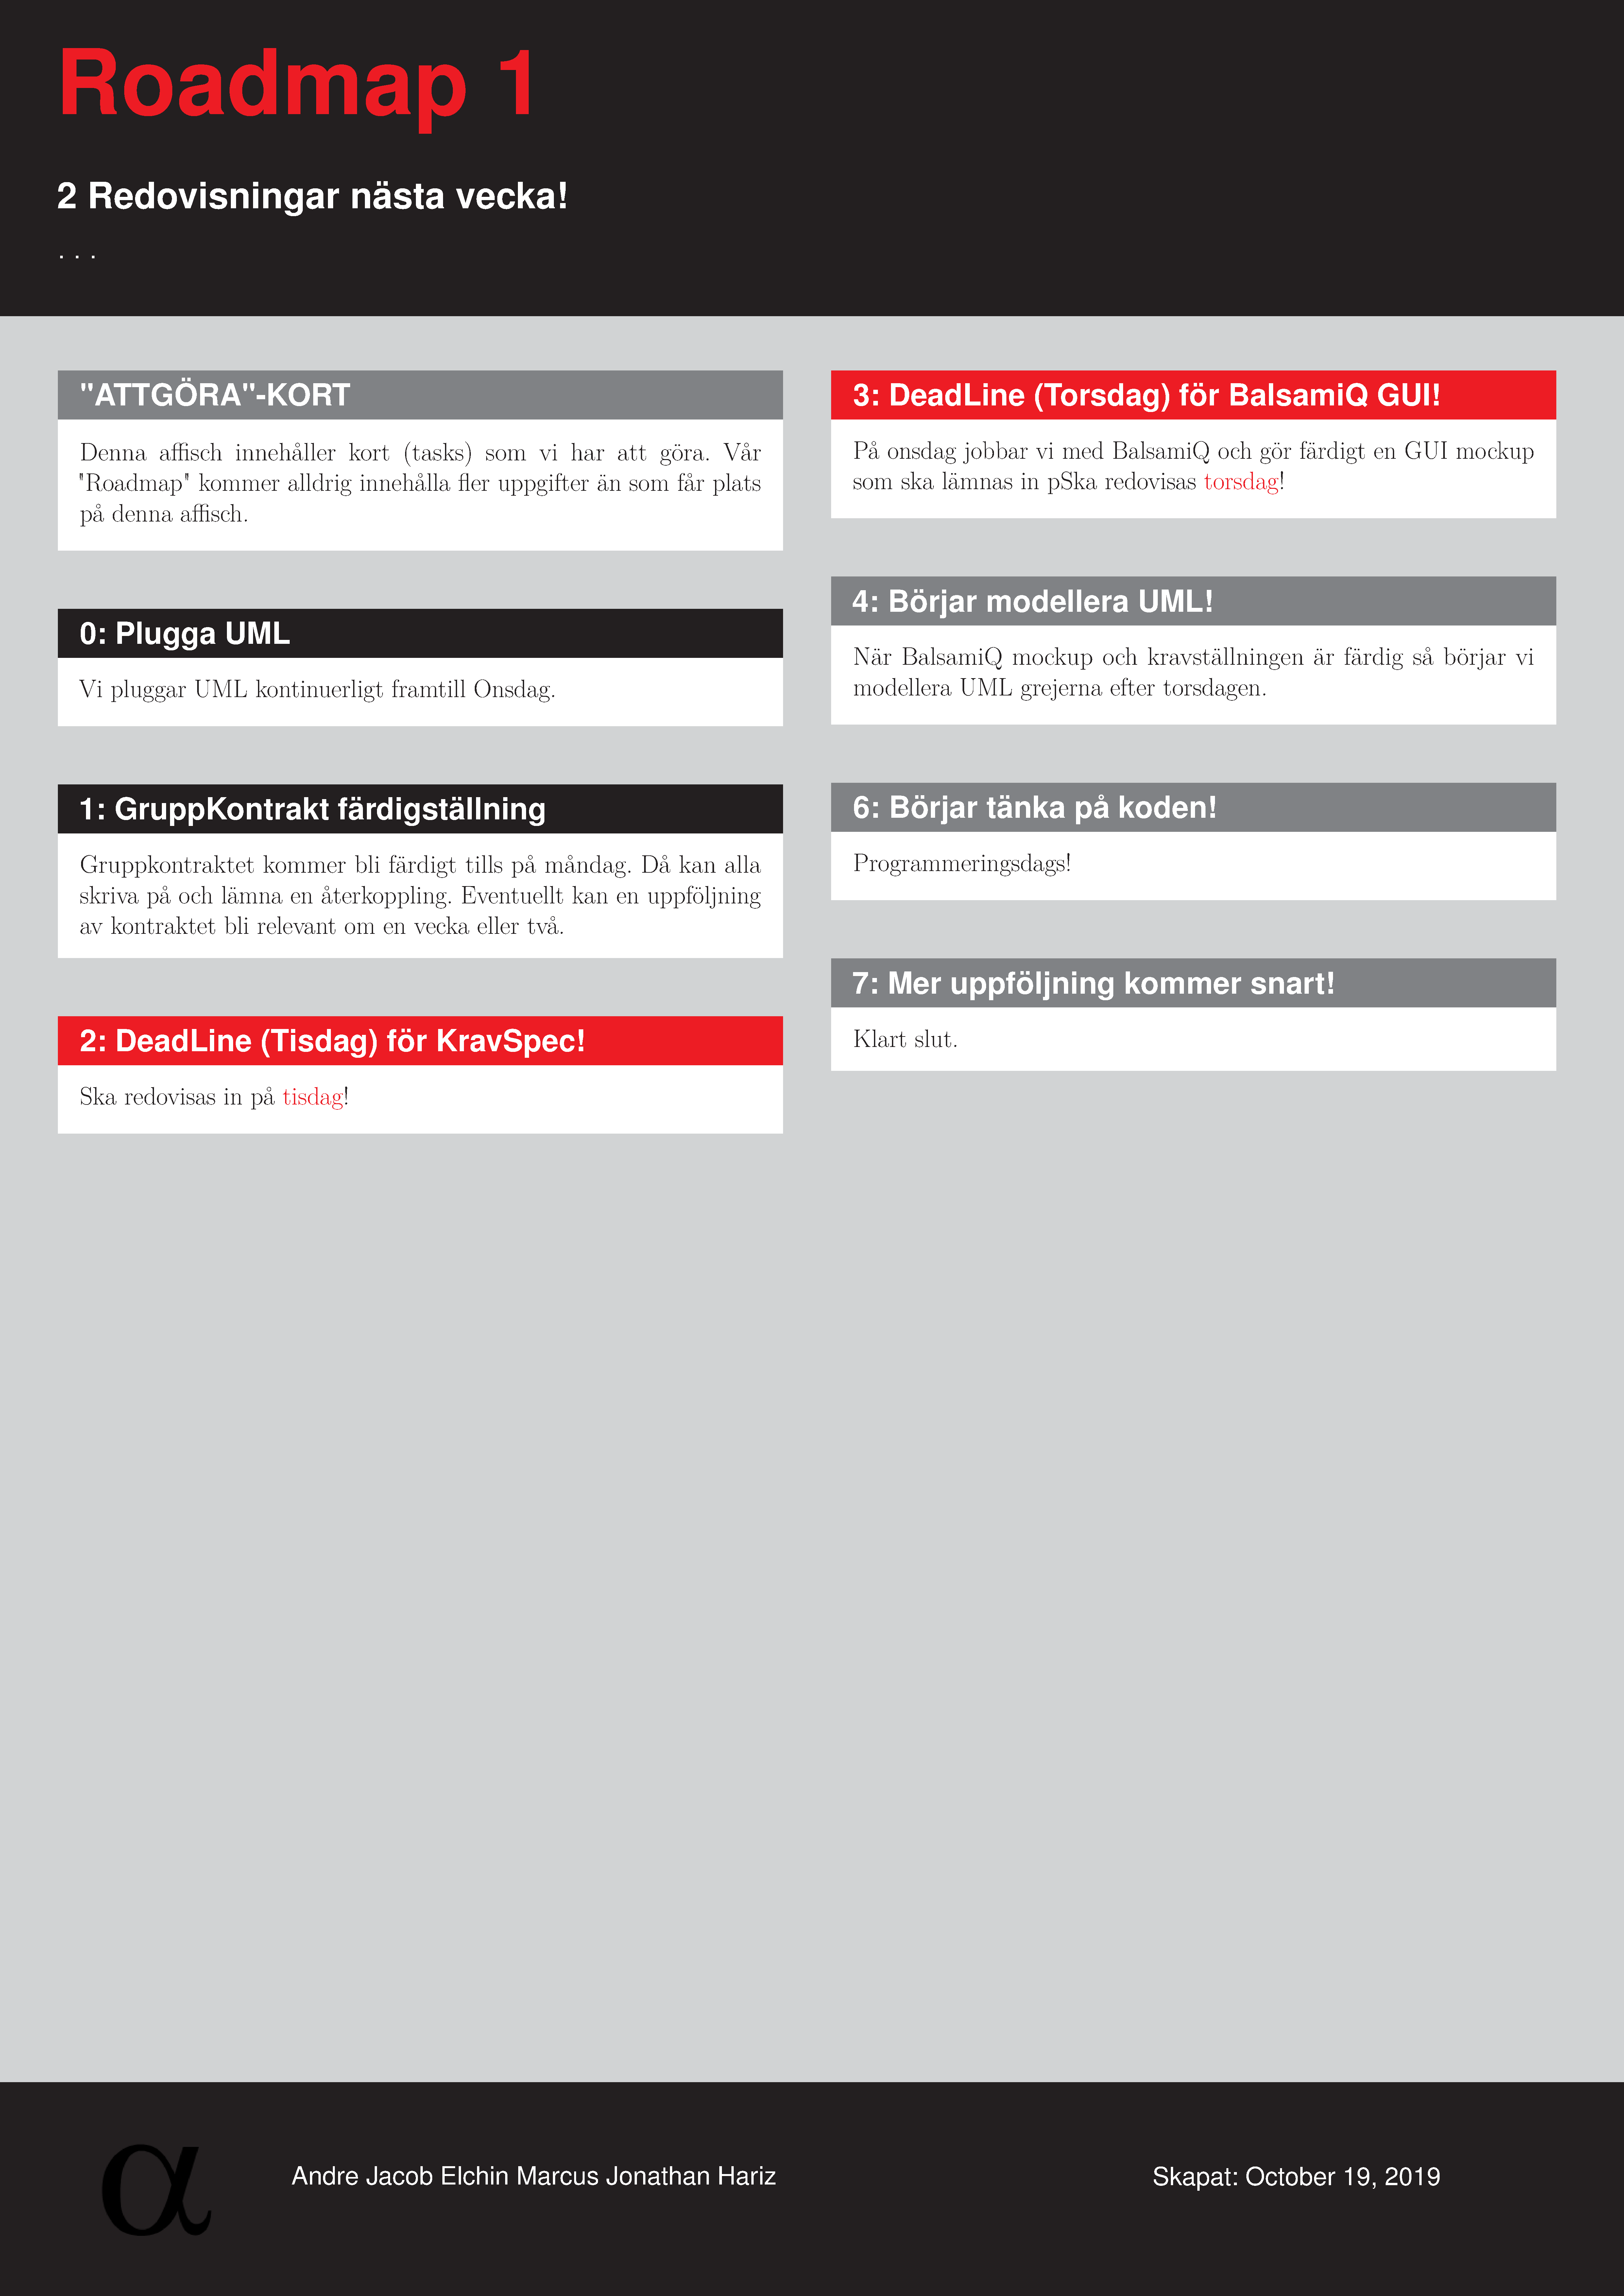
\includegraphics[width=\textwidth]{img/OBJKURS1_Roadmap.pdf}
        \caption{Roadmap1}
        \label{fig:road1}
    \end{subfigure}
    \begin{subfigure}[b]{0.3\textwidth}
        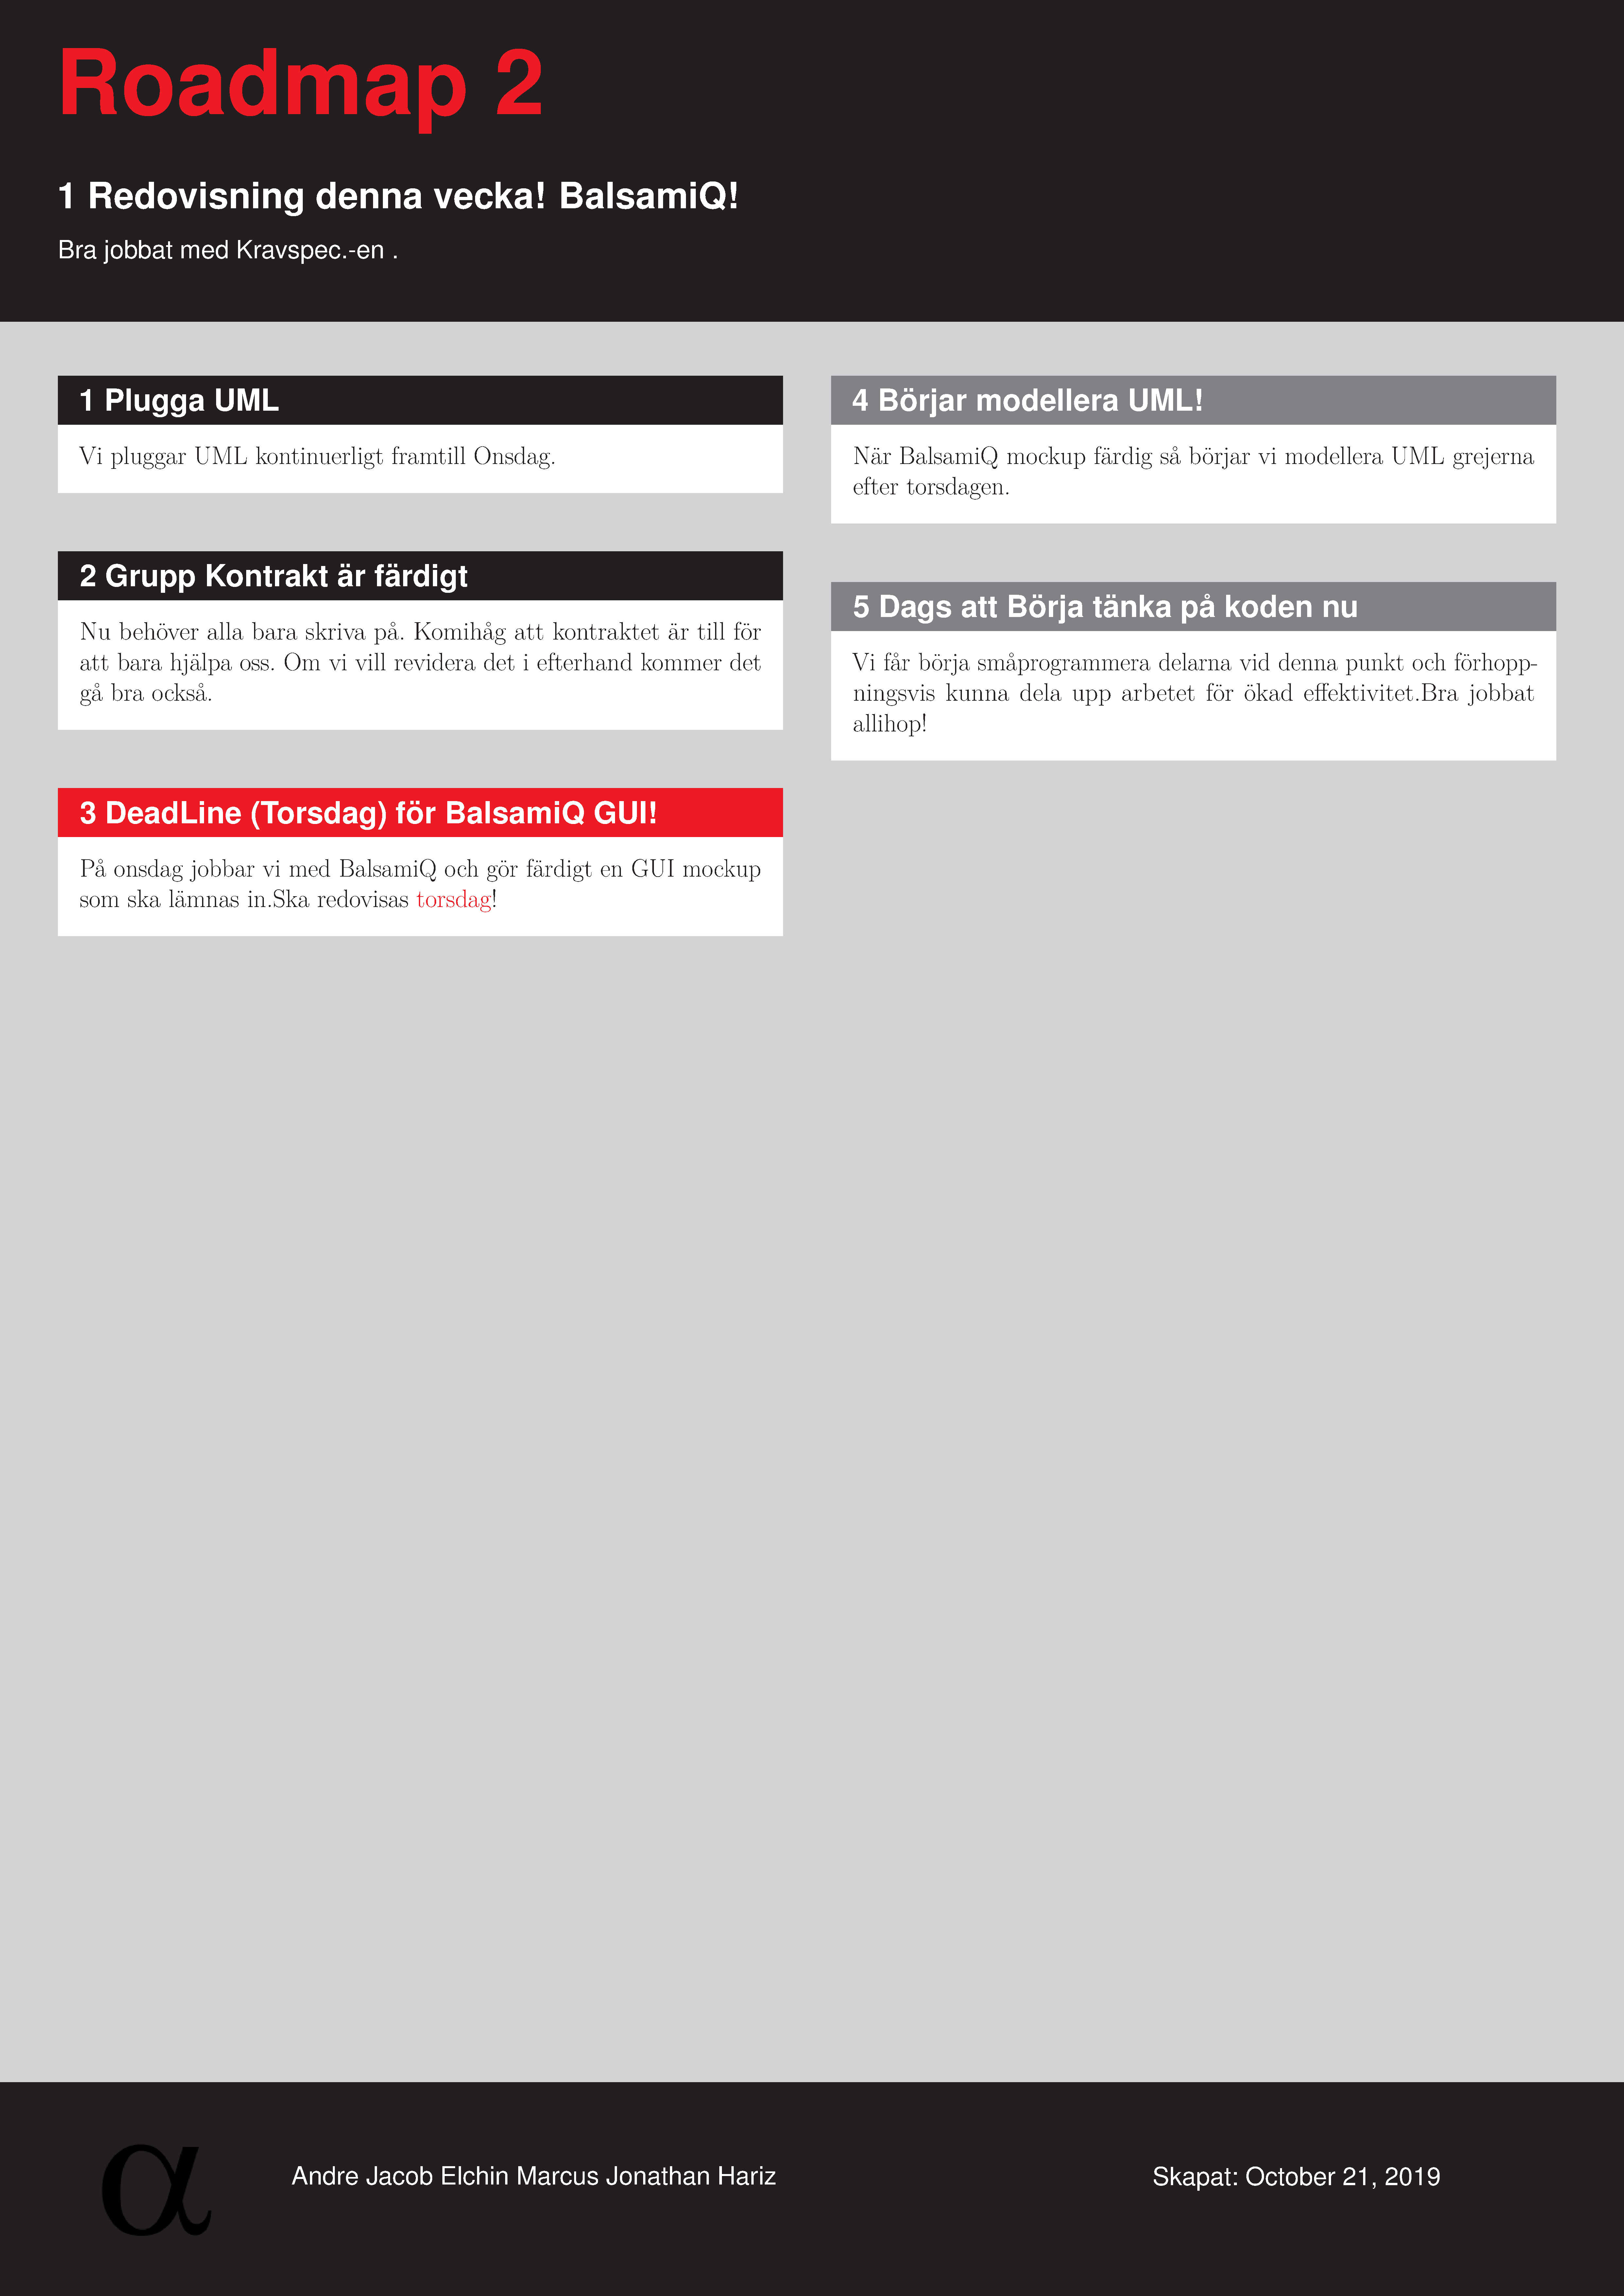
\includegraphics[width=\textwidth]{img/OBJKURS1_Roadmap2.pdf}
        \caption{Roadmap2}
        \label{fig:road2}
    \end{subfigure}
    \begin{subfigure}[b]{0.3\textwidth}
        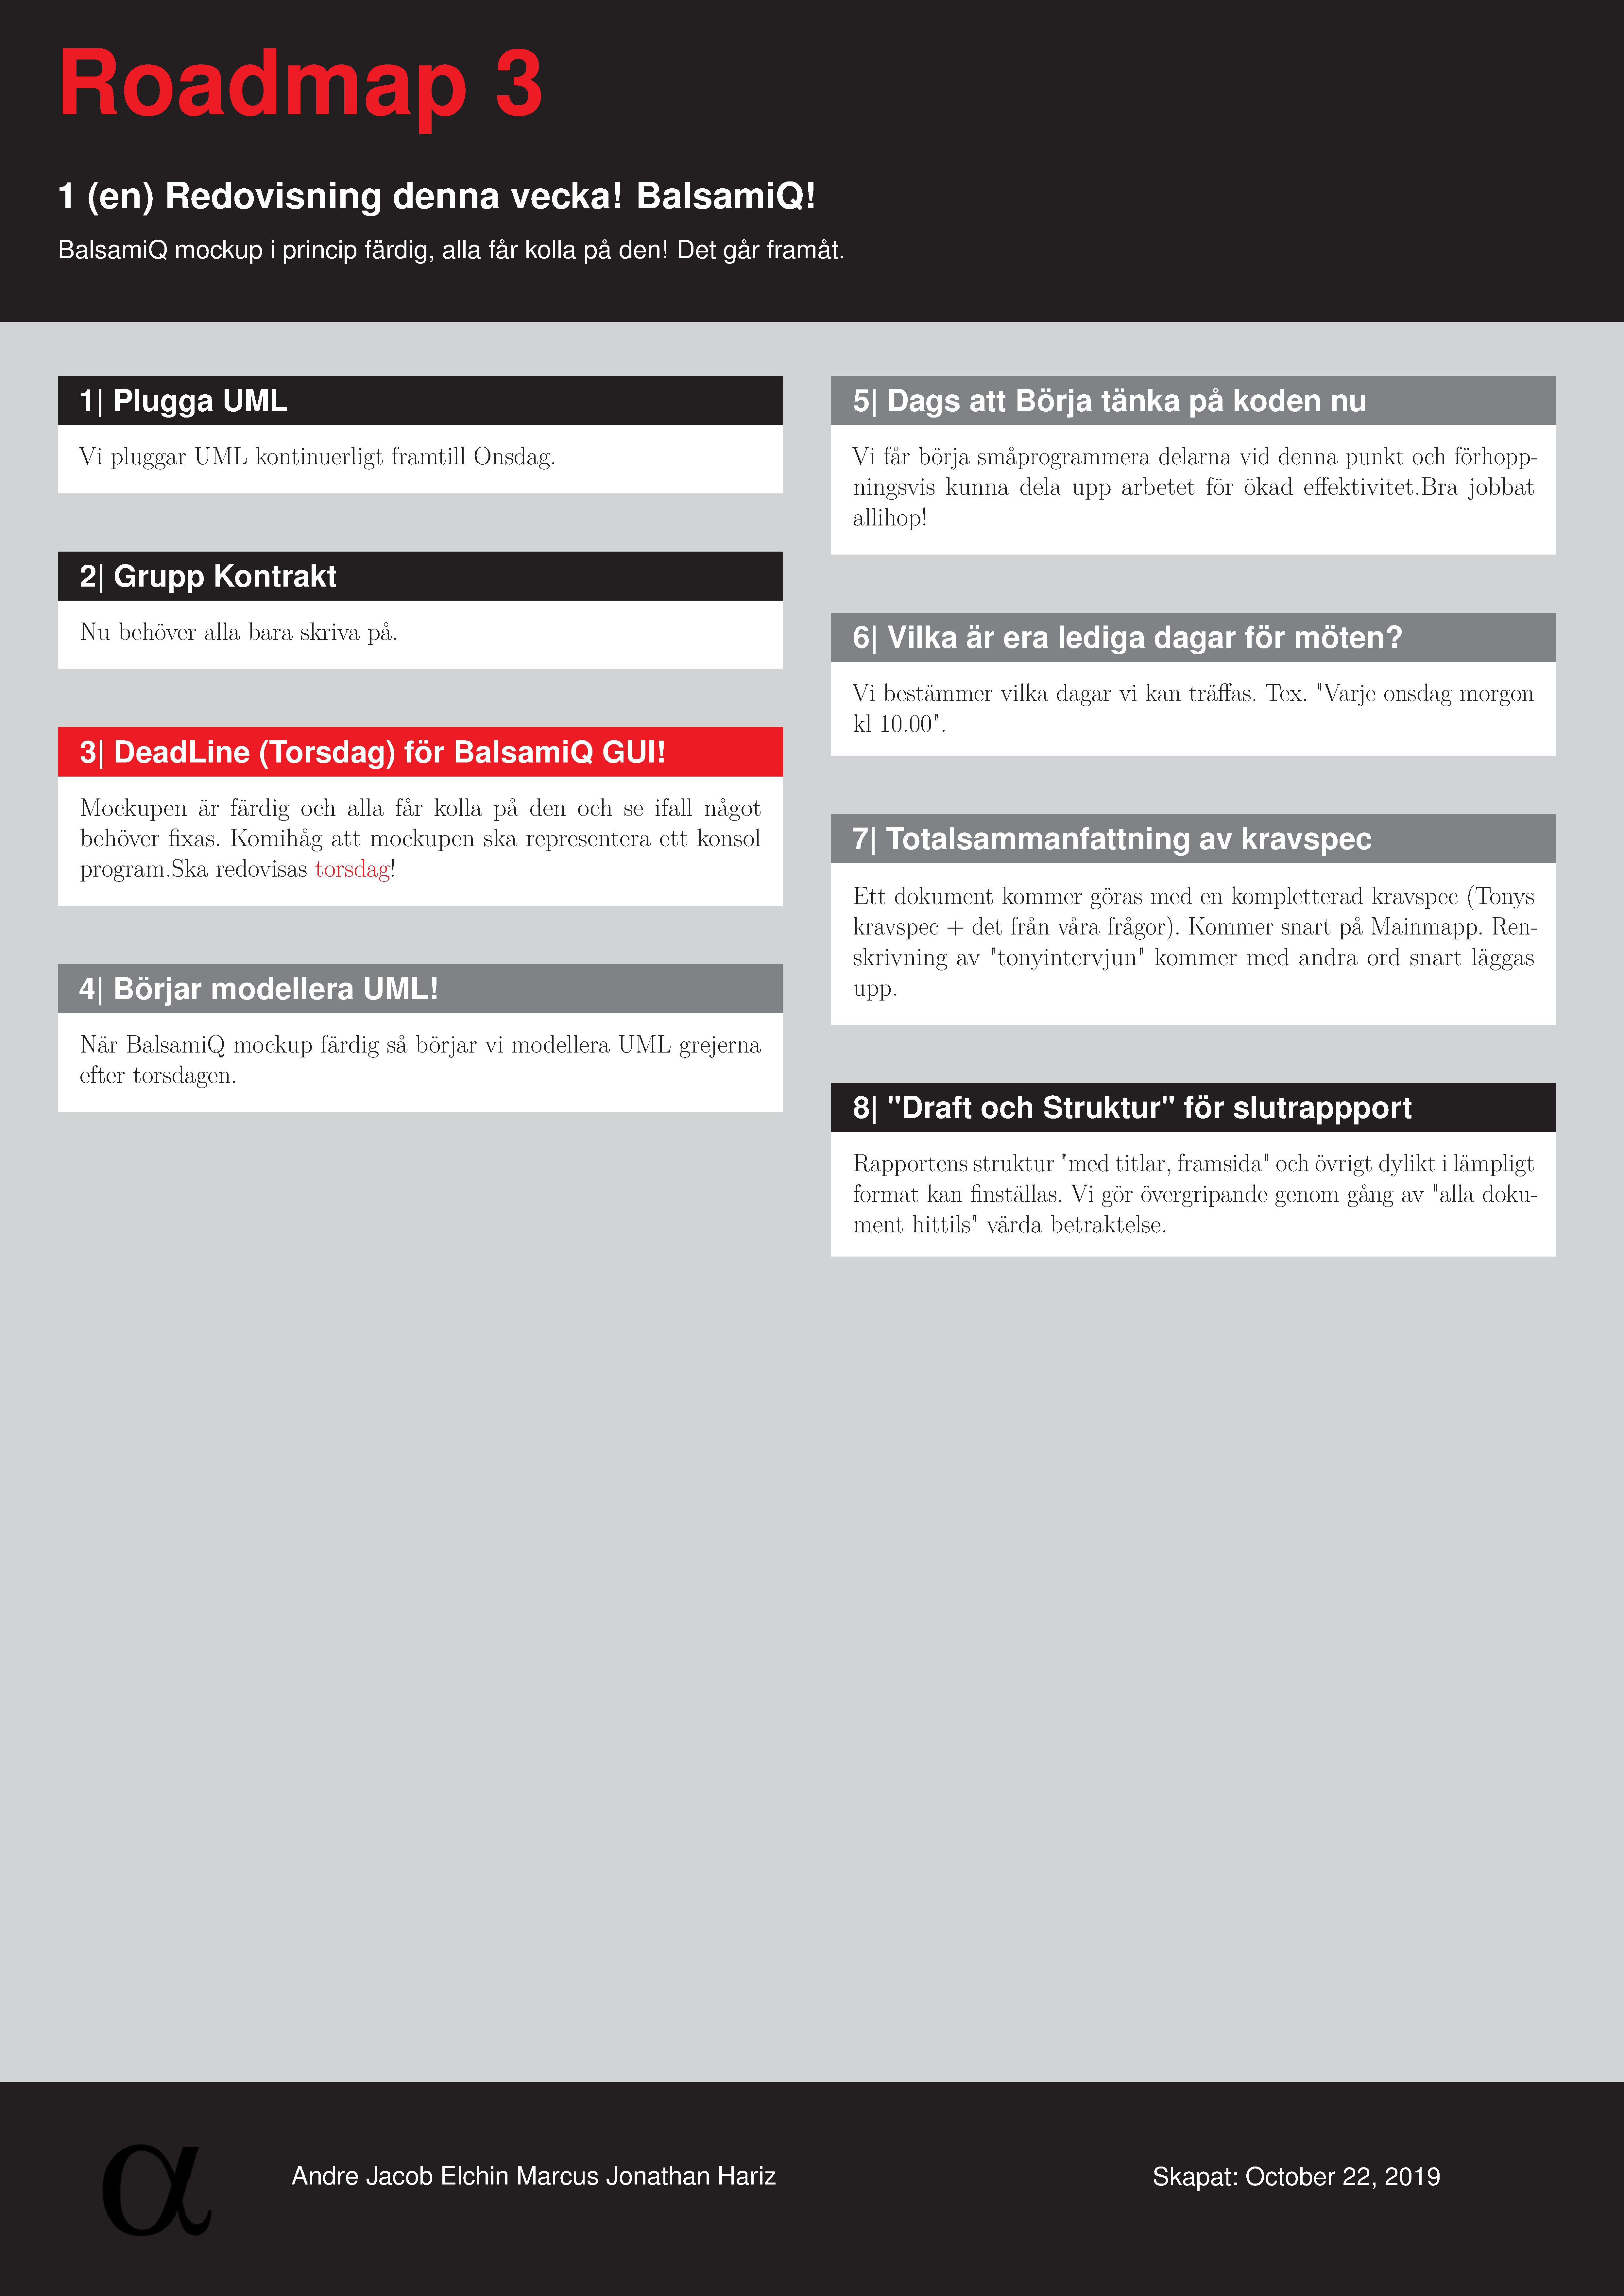
\includegraphics[width=\textwidth]{img/OBJKURS1_Roadmap3.pdf}
        \caption{Roadmap3}
        \label{fig:road3}
    \end{subfigure}
    \begin{subfigure}[b]{0.3\textwidth}
        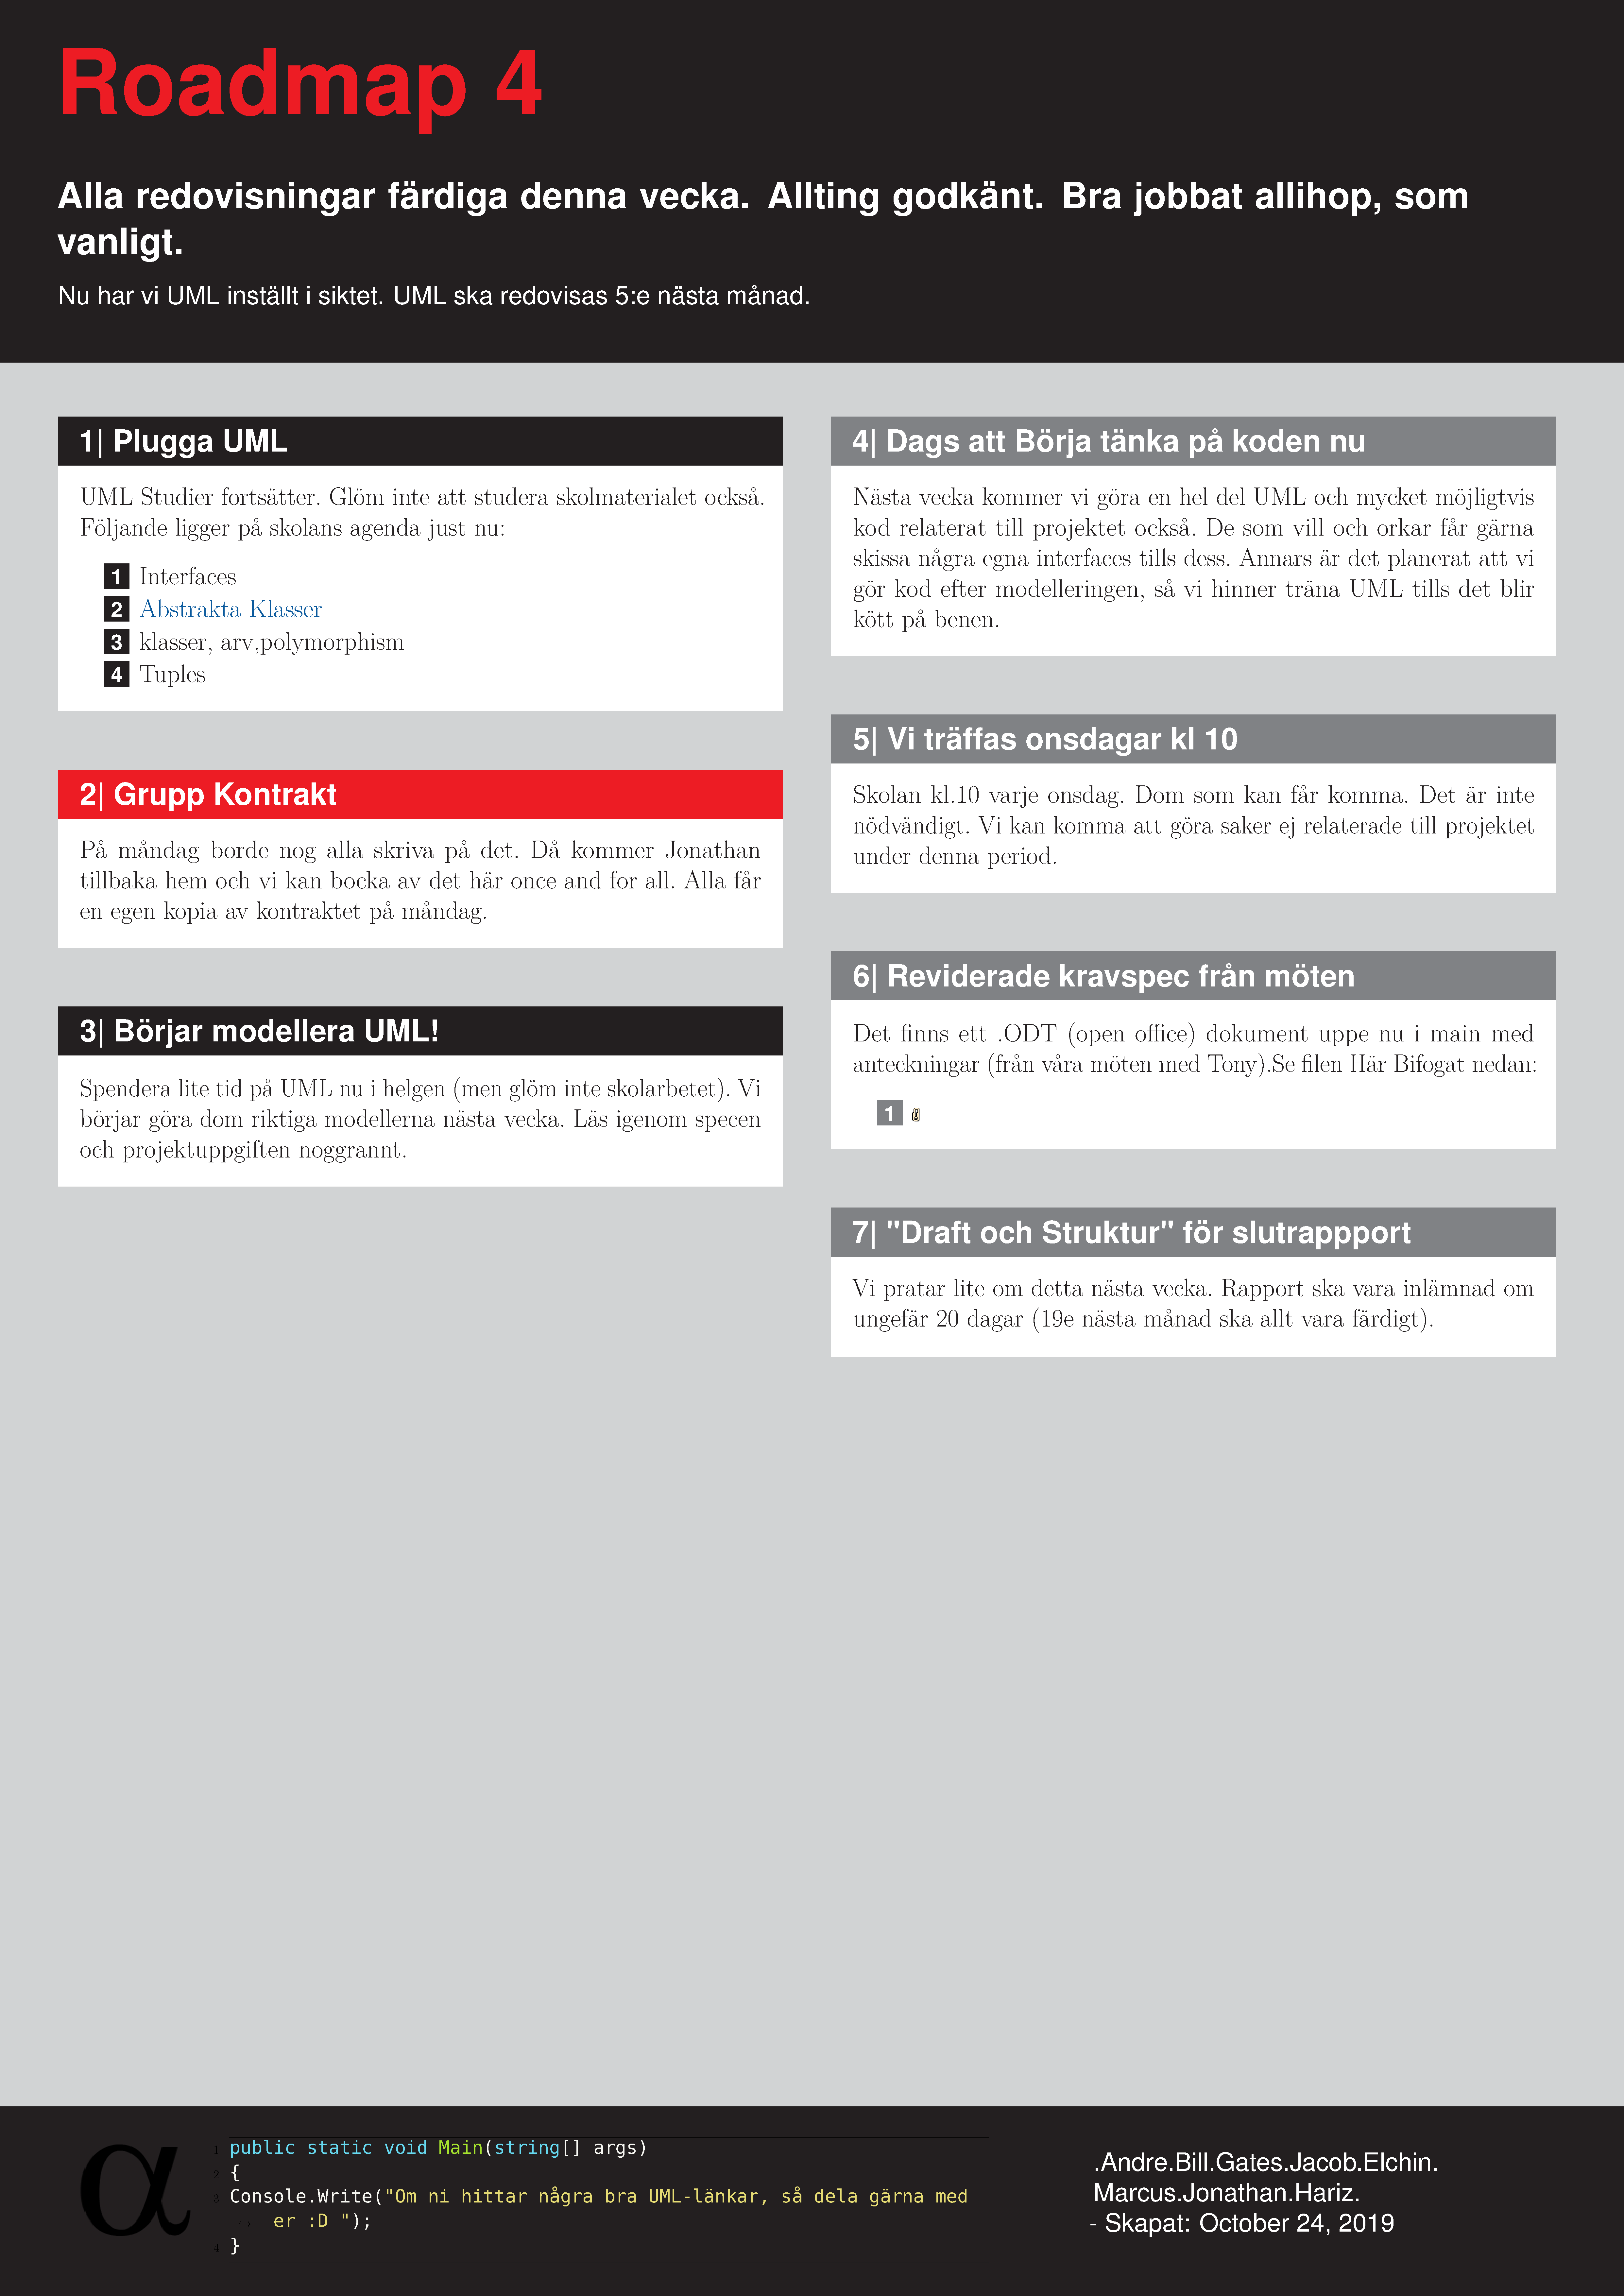
\includegraphics[width=\textwidth]{img/Roadmap4.pdf}
        \caption{Roadmap4}
        \label{fig:road4}
    \end{subfigure}    
    \begin{subfigure}[b]{0.3\textwidth}
        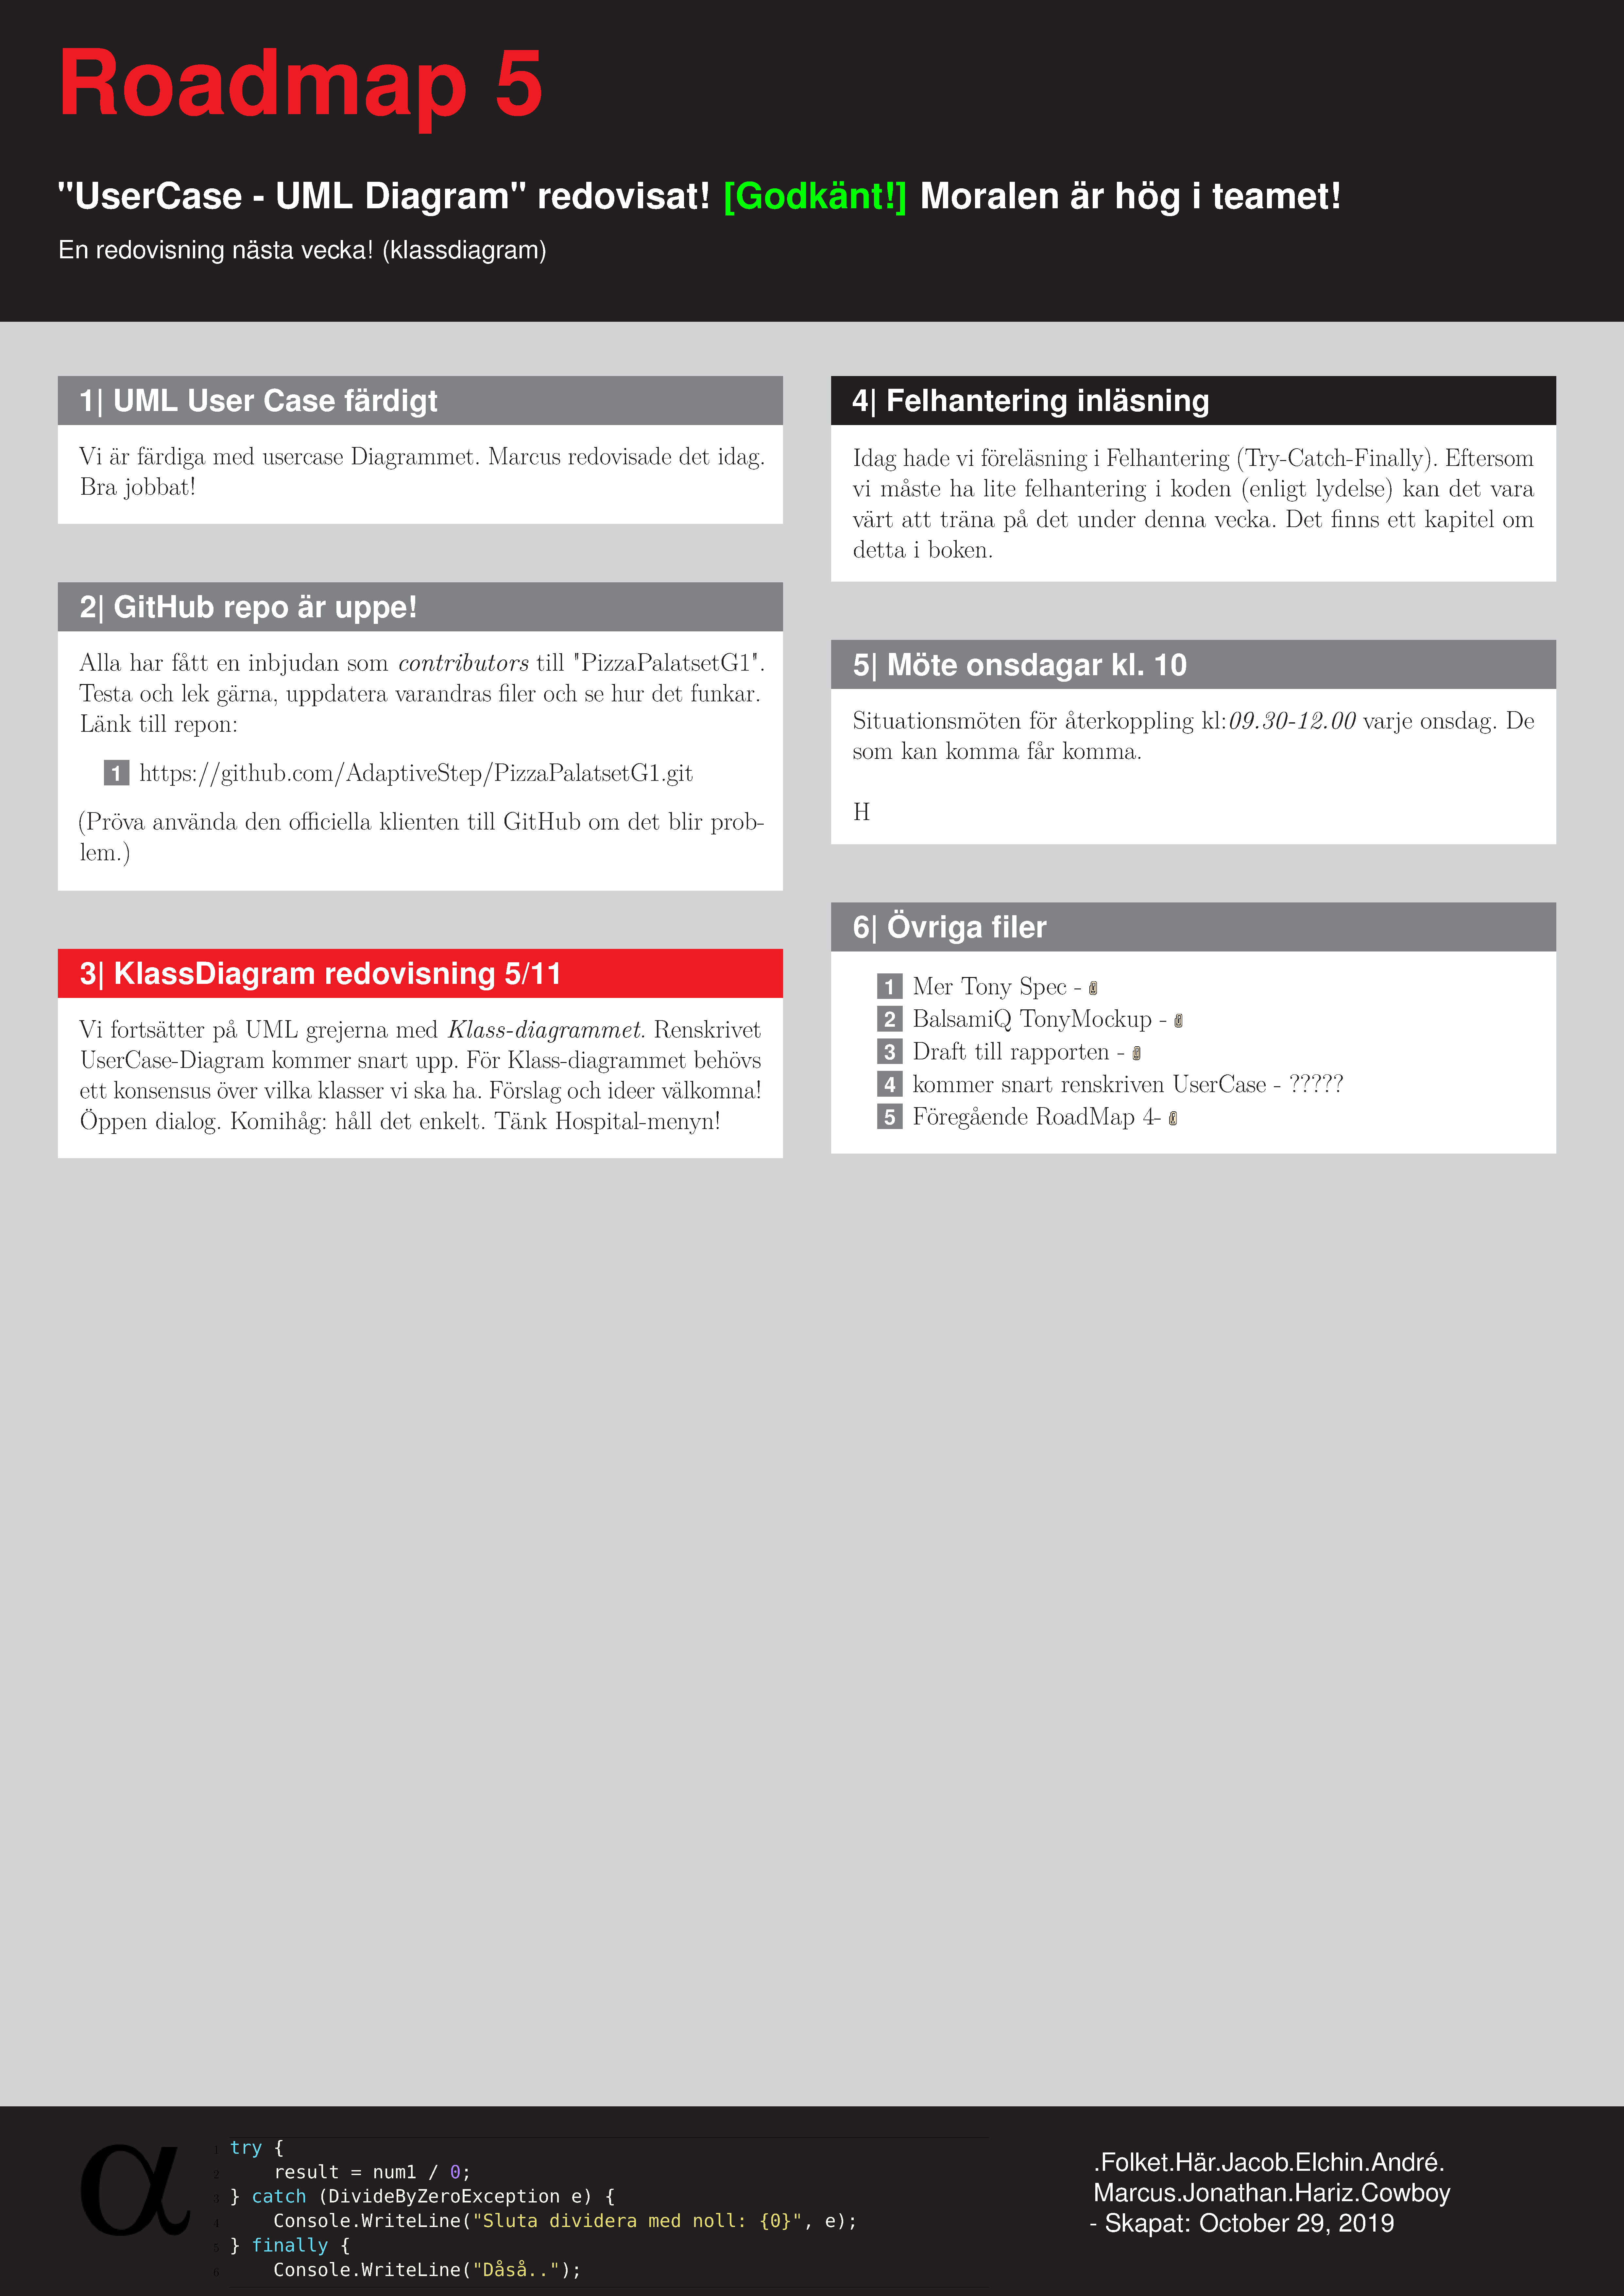
\includegraphics[width=\textwidth]{img/Roadmap5.pdf}
        \caption{Roadmap5}
        \label{fig:road5}
    \end{subfigure}    
    \begin{subfigure}[b]{0.3\textwidth}
        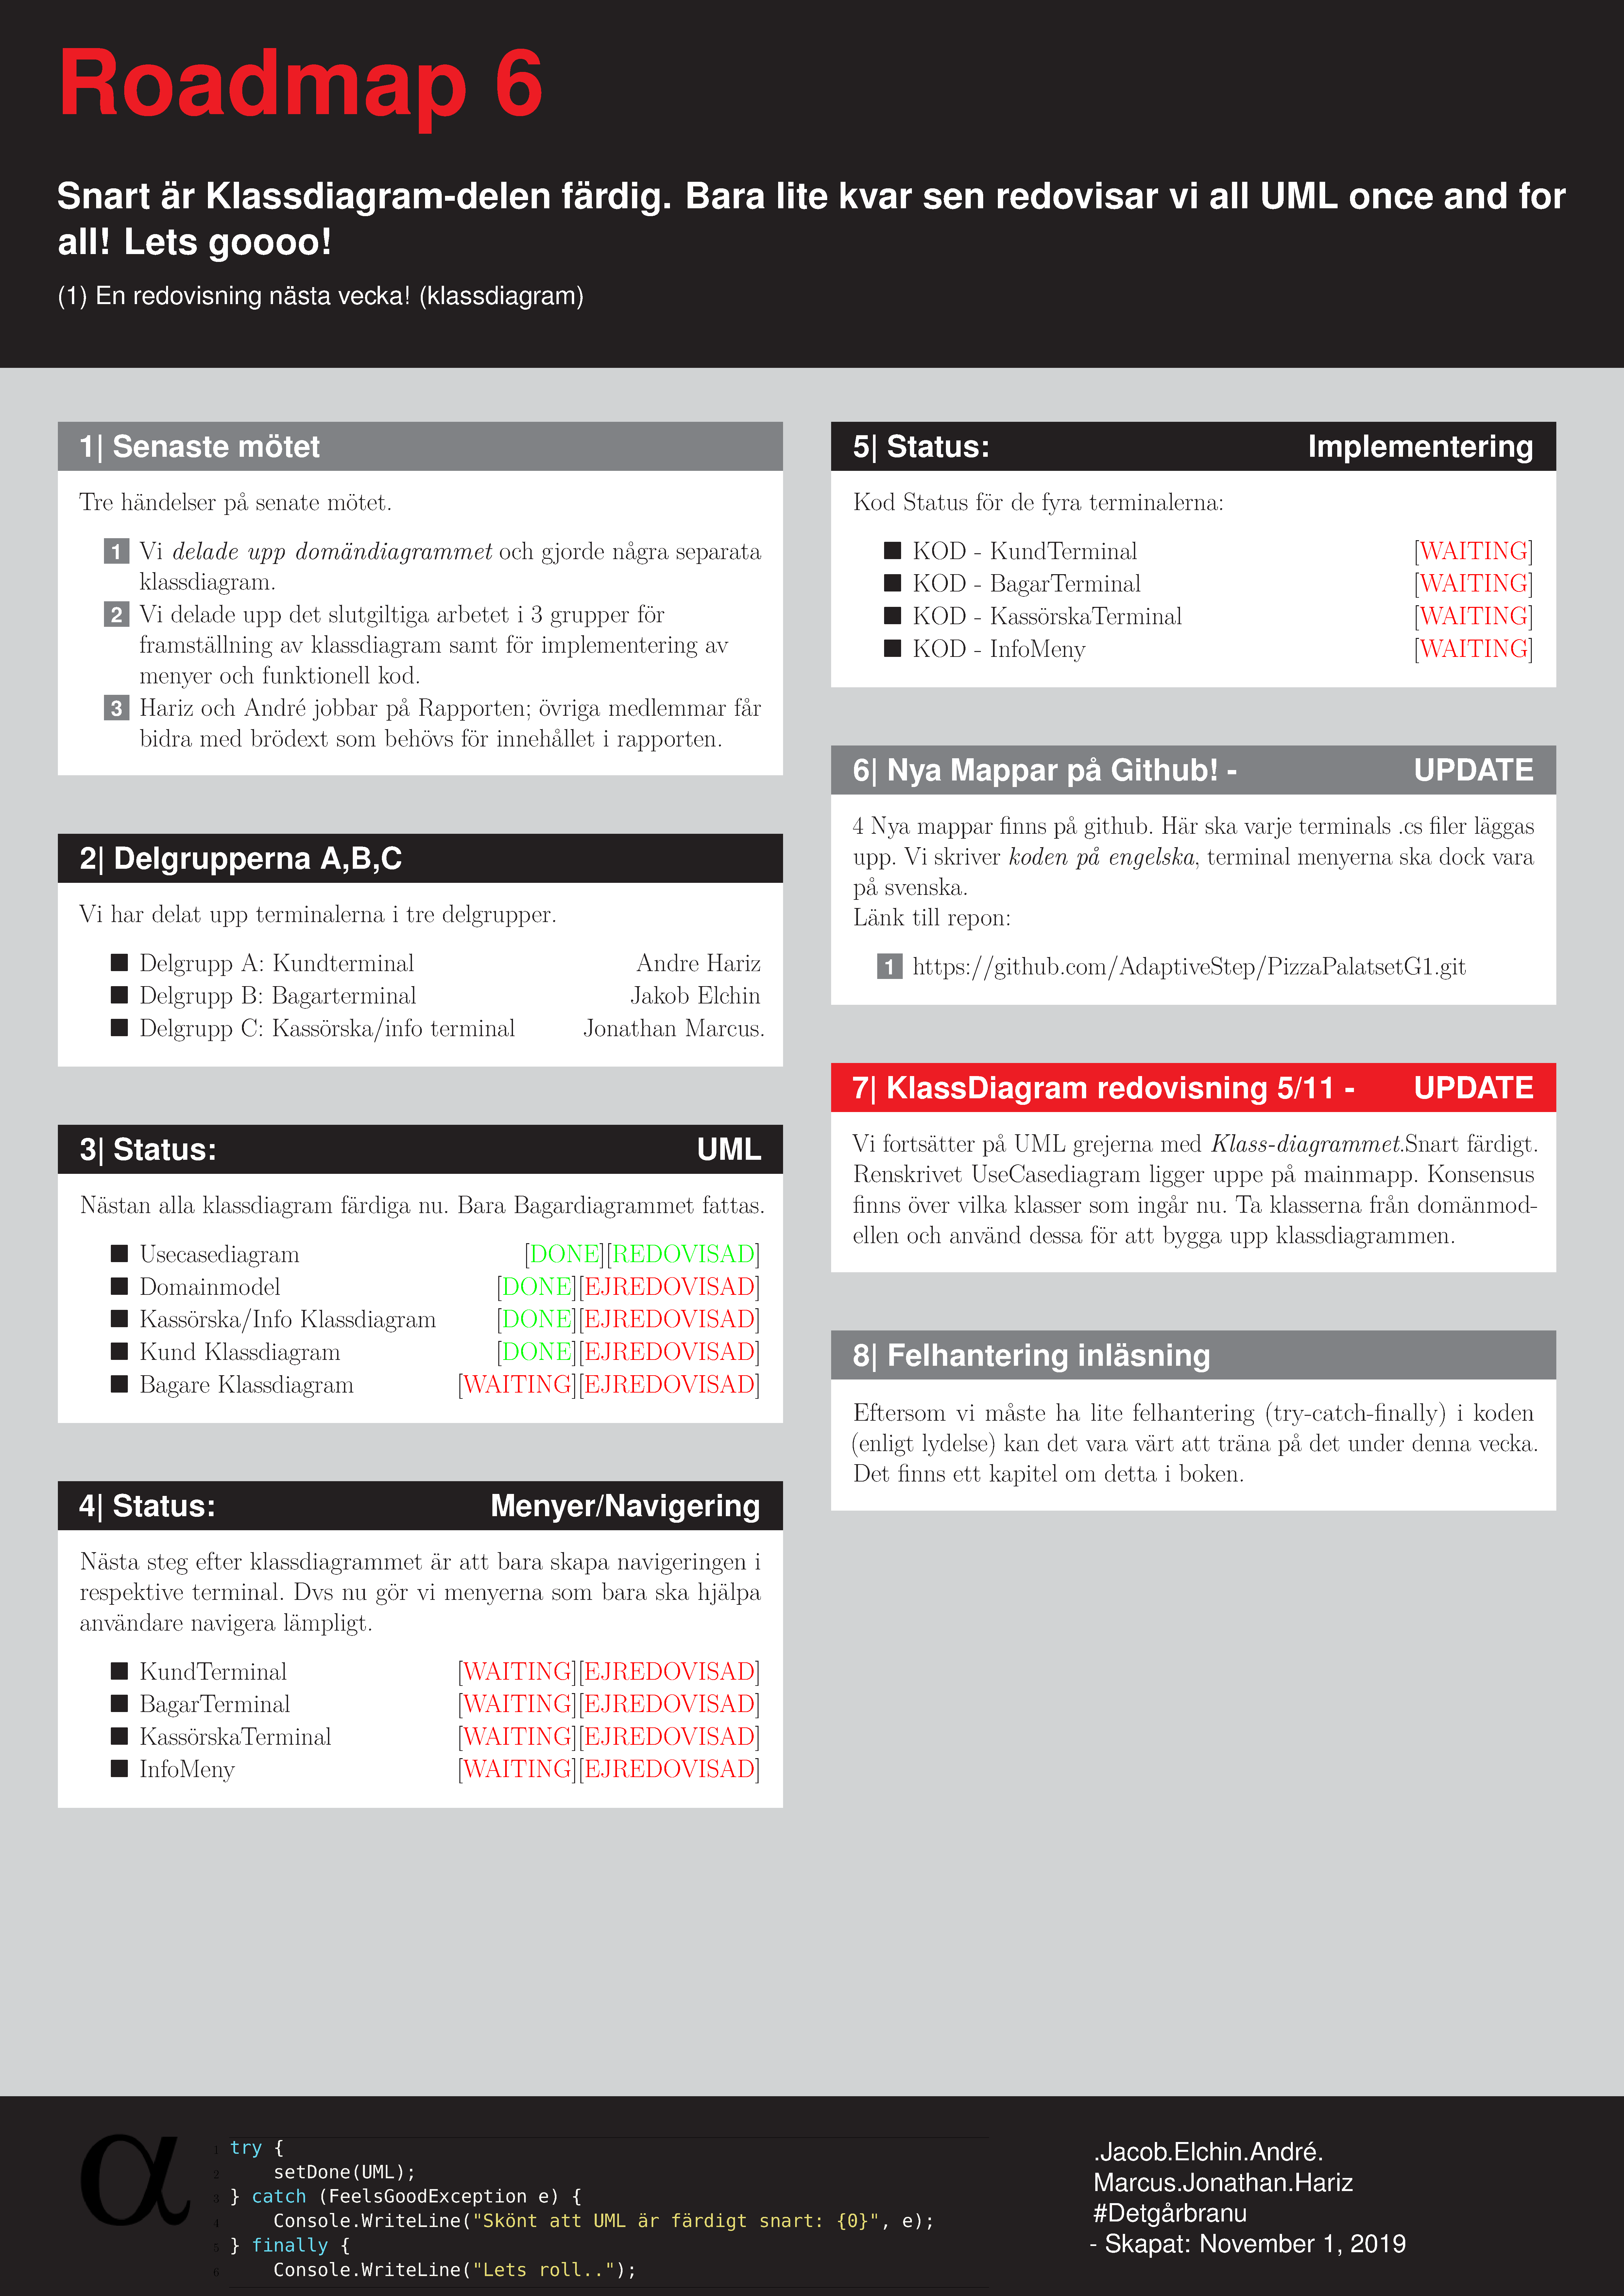
\includegraphics[width=\textwidth]{img/Roadmap6.pdf}
        \caption{Roadmap6}
        \label{fig:road6}
    \end{subfigure}    
    \begin{subfigure}[b]{0.3\textwidth}
        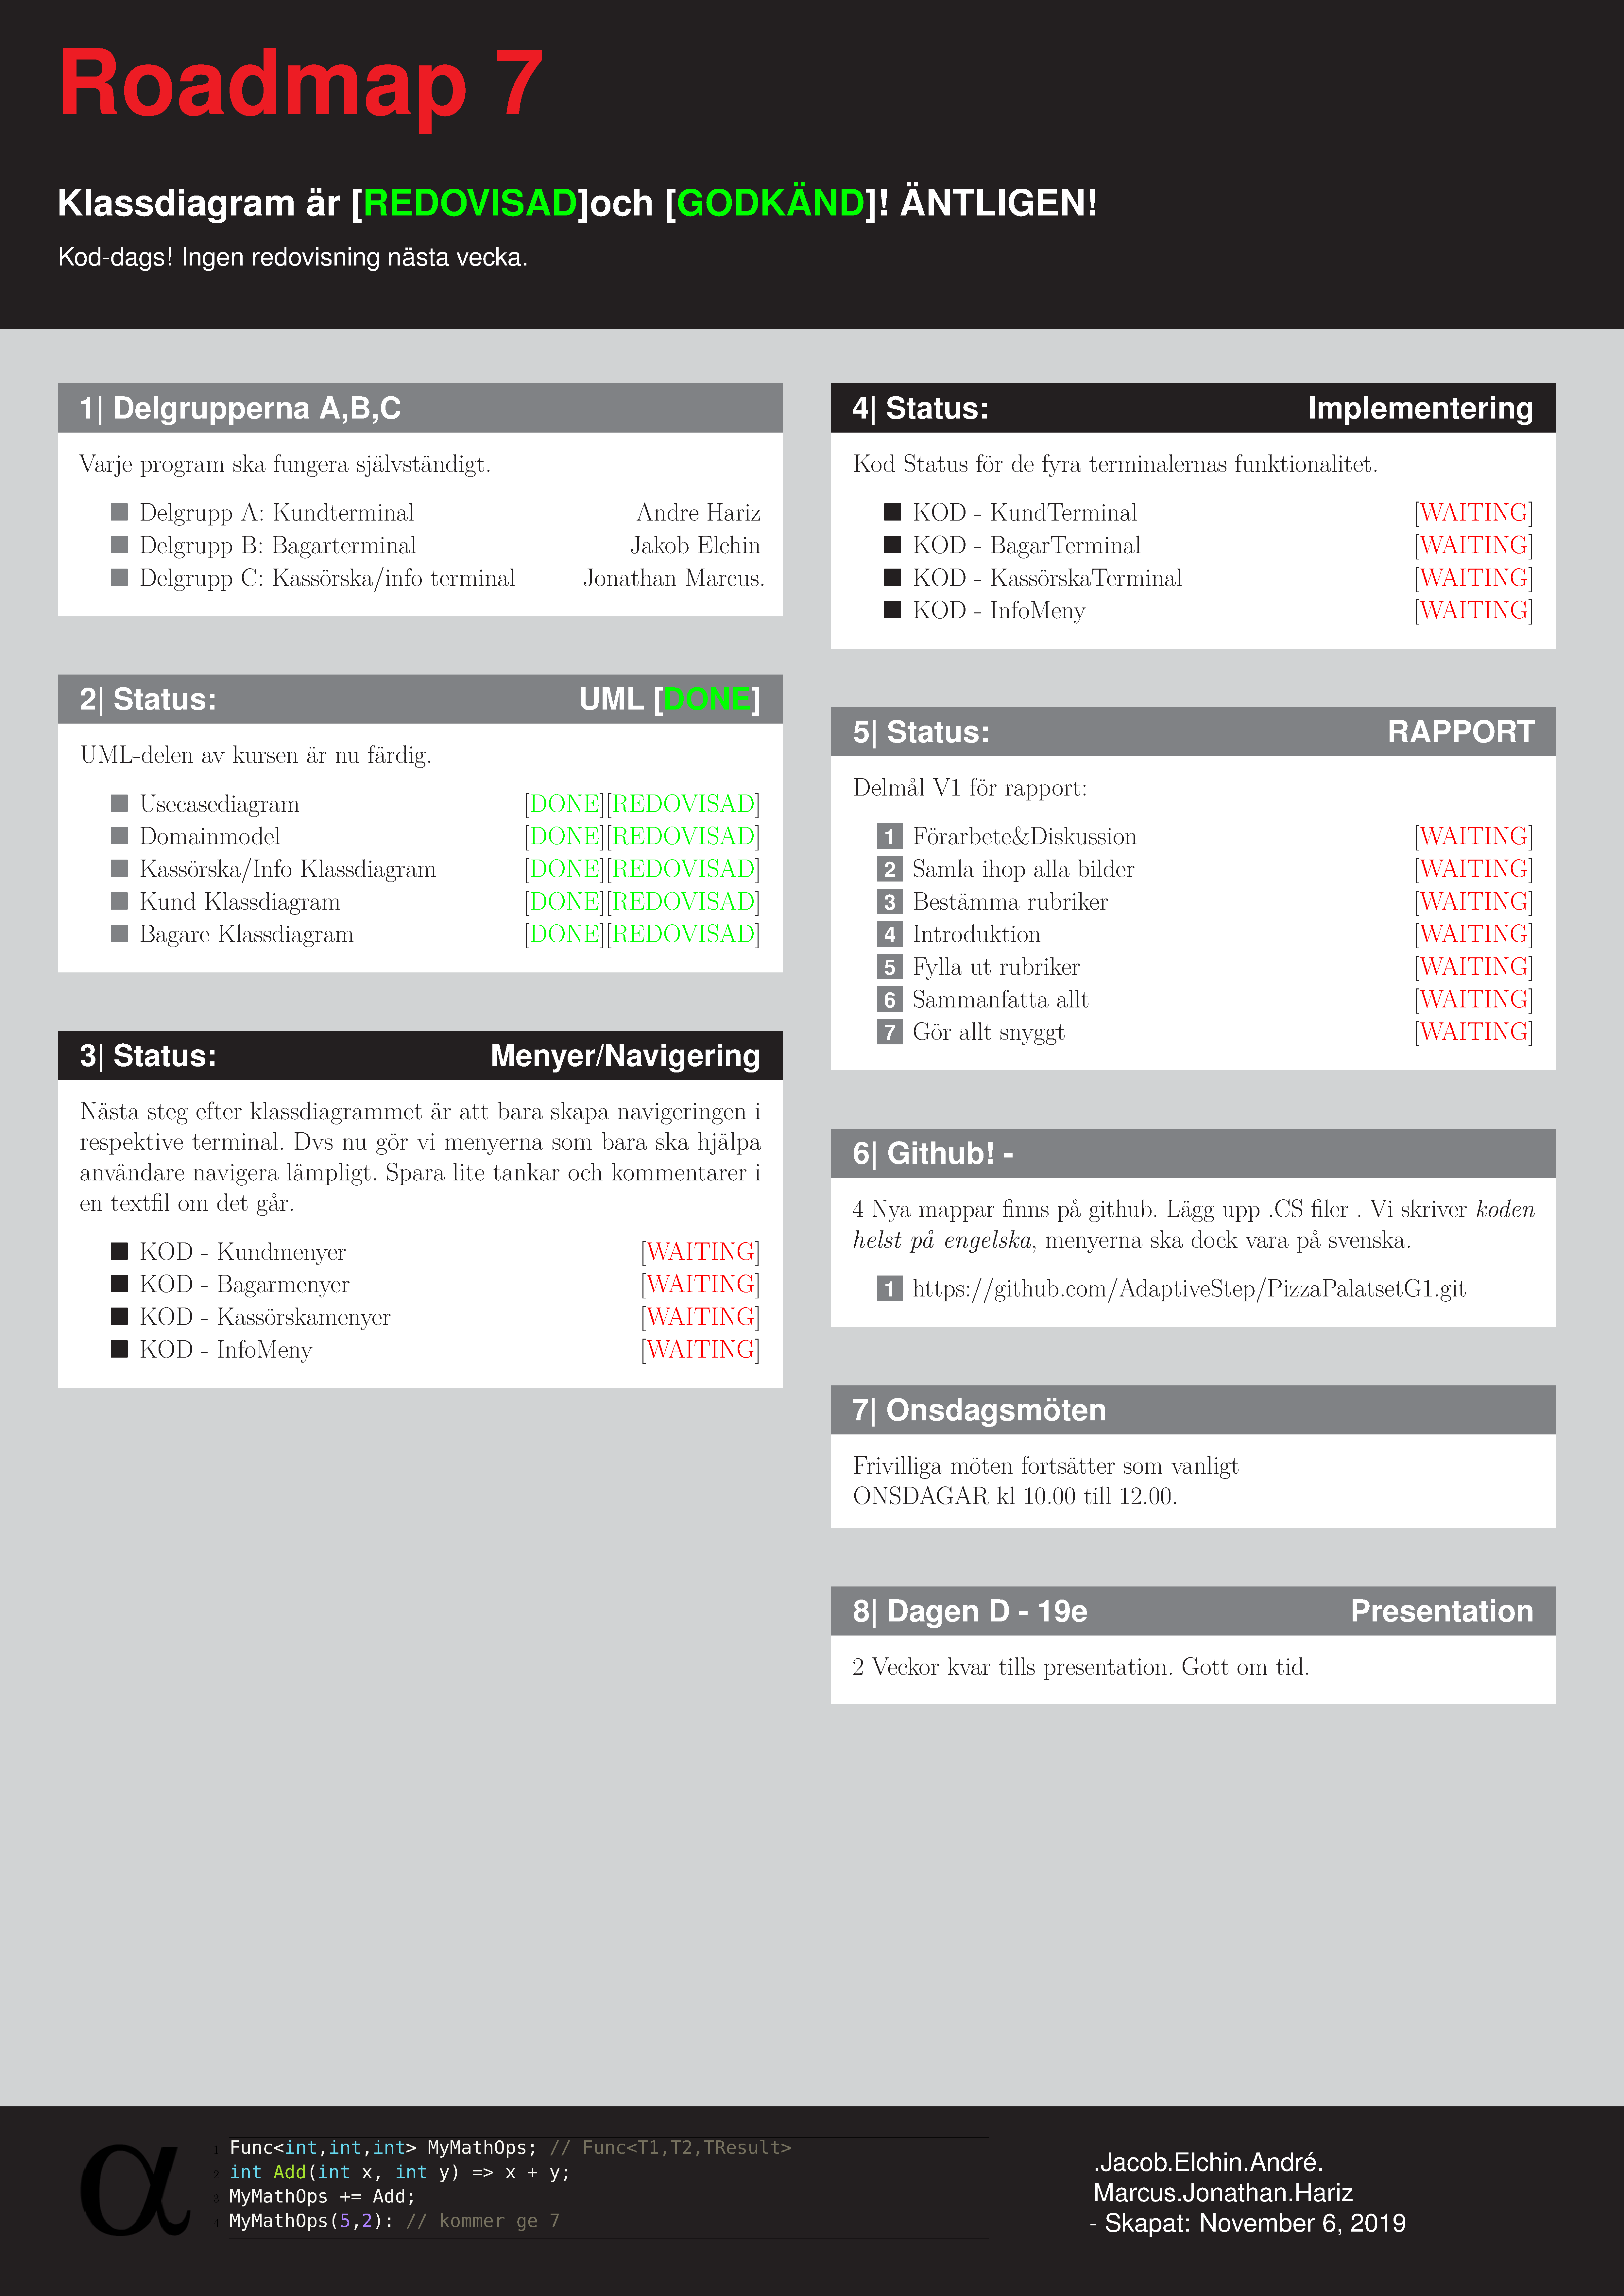
\includegraphics[width=\textwidth]{img/Roadmap7.pdf}
        \caption{Roadmap7}
        \label{fig:road7}
    \end{subfigure}    
    \begin{subfigure}[b]{0.3\textwidth}
        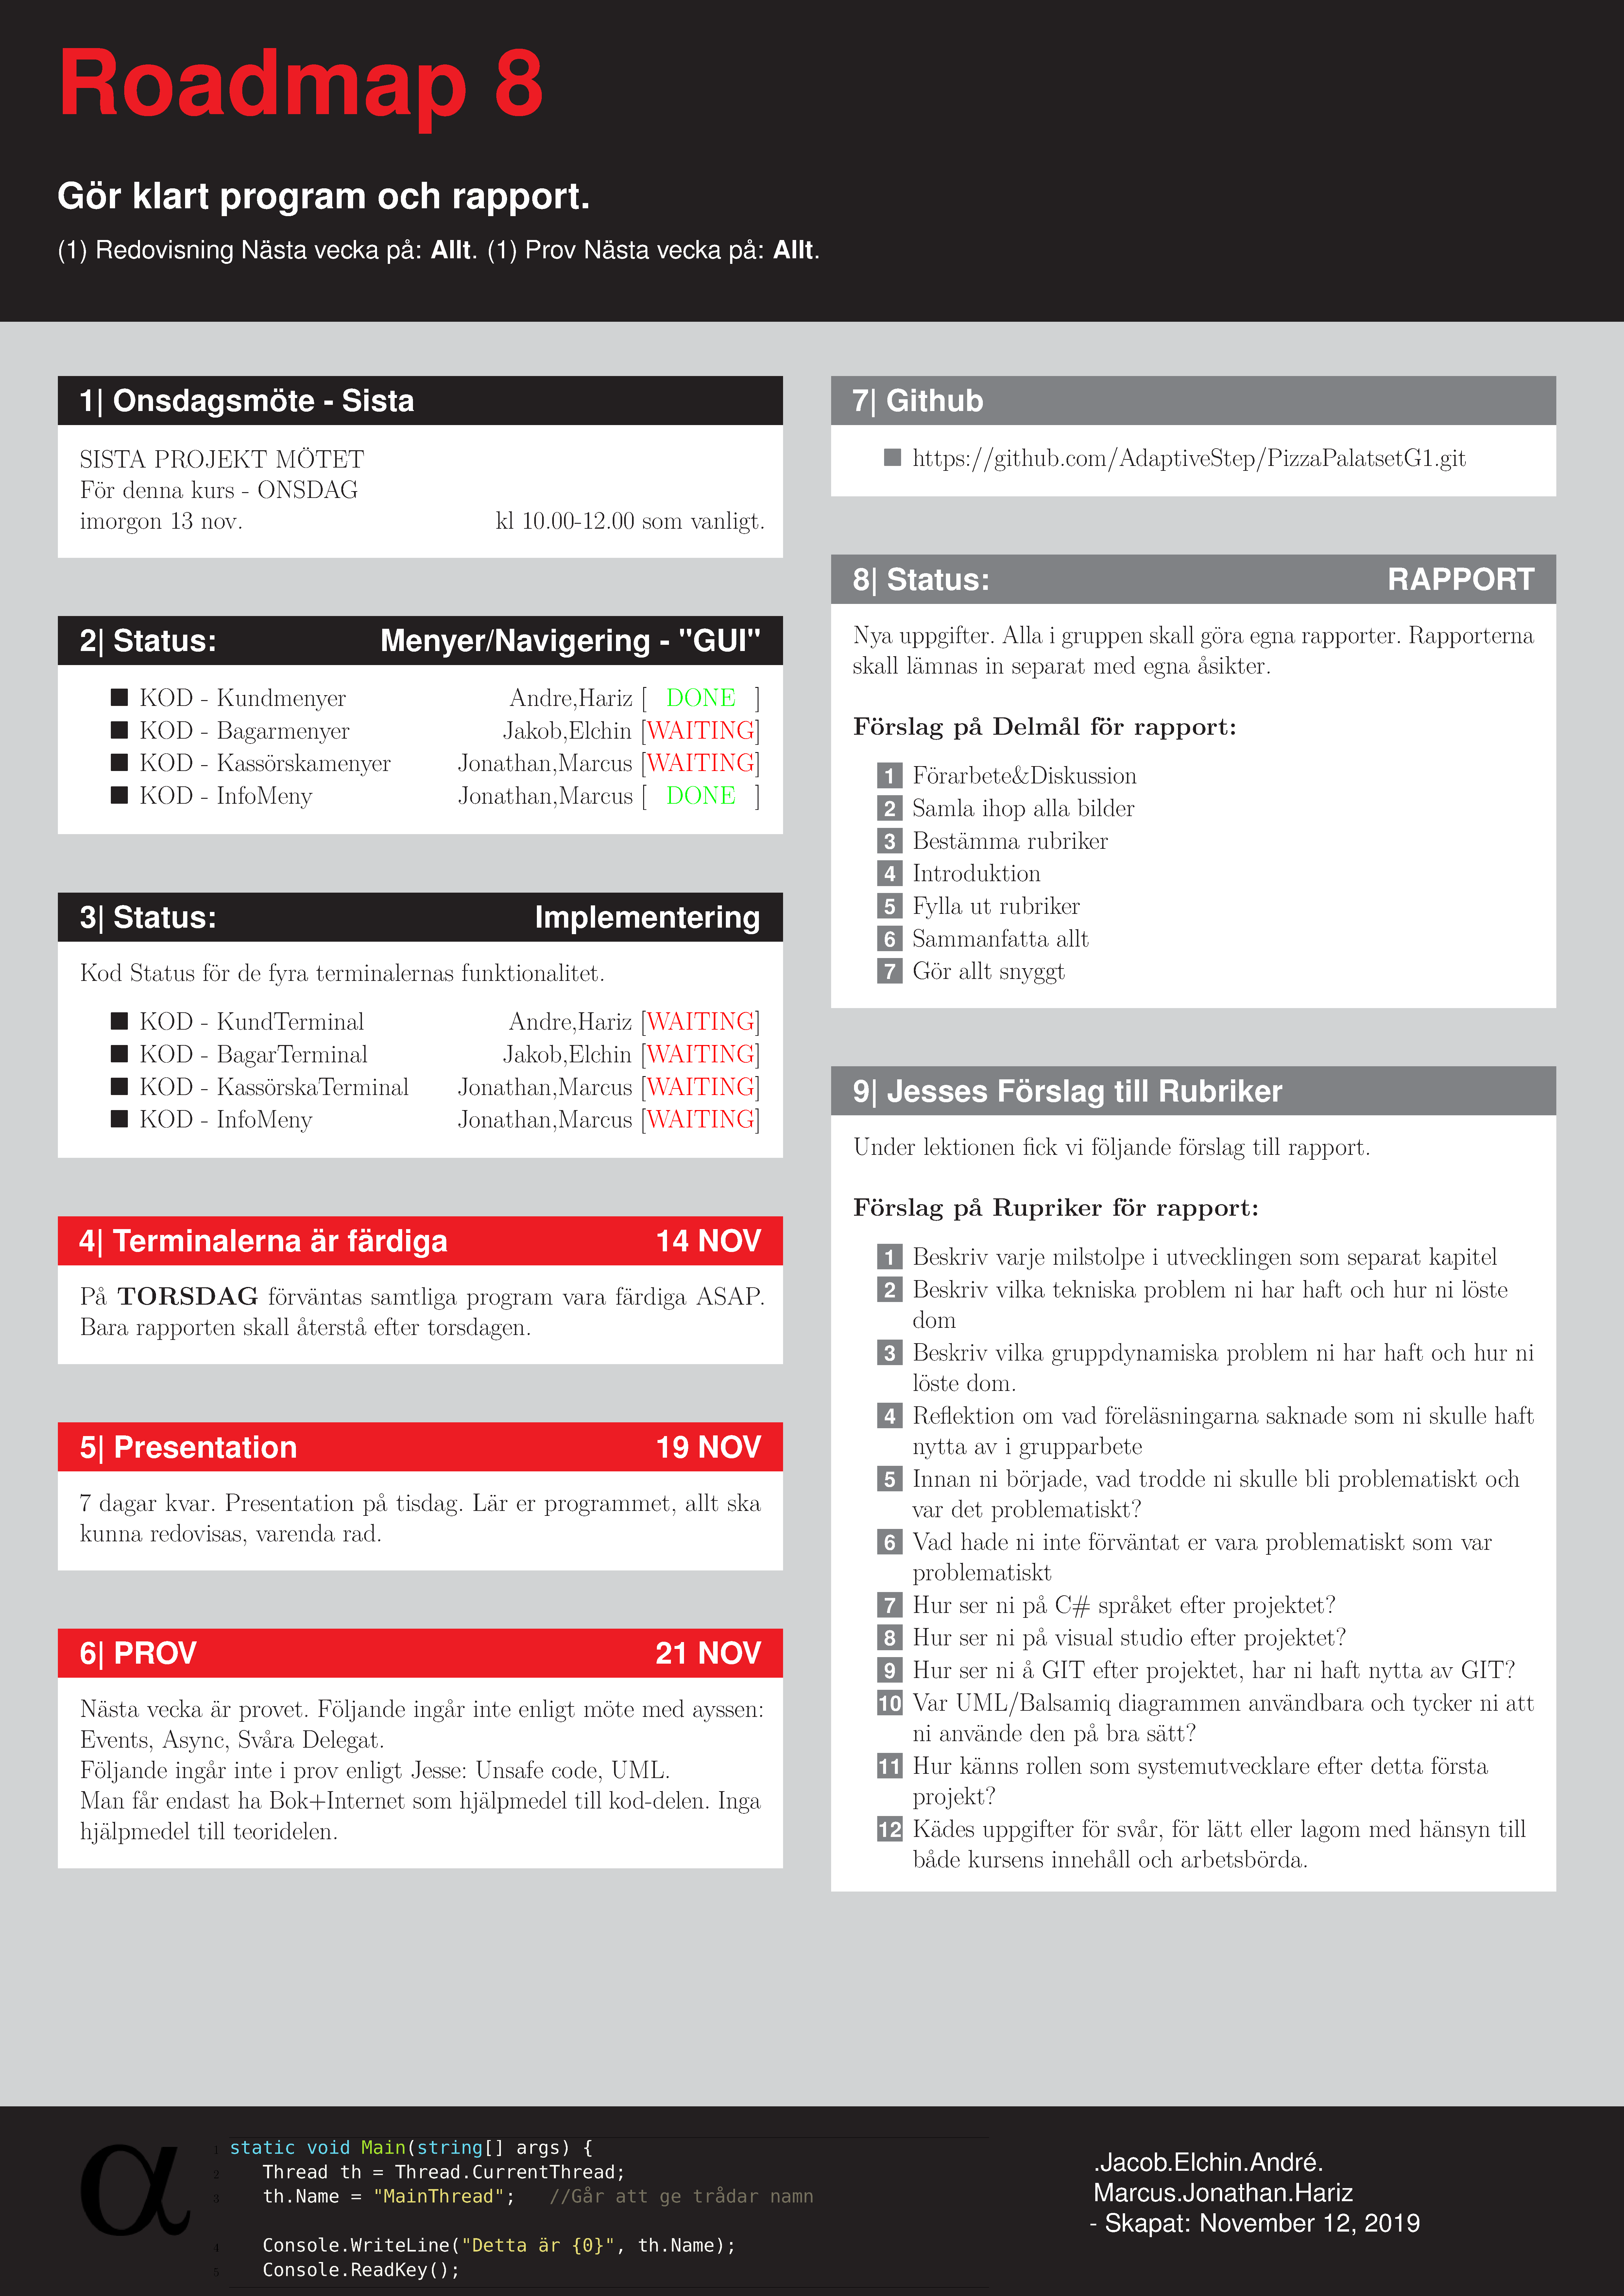
\includegraphics[width=\textwidth]{img/Roadmap8.pdf}
        \caption{Roadmap8}
        \label{fig:road8}
    \end{subfigure}    
    \caption{Bilder av våra Roadmaps som delades ut genom hela projektet}\label{fig:Roadmaps}
\end{figure}

Under huvudarbetet hade vi försås många föreläsningar vilka hjälpte till att hålla vår grupp i fas (möjligtvis på grund av en känsla av brådskan). Trots lärarnas ambition och samverkan med eleverna bör nog respektfullt följande notering anmärkas: \emph{projektets lydelse uppfattades som motsägande från främst den informationen vi fick från lärarna}. Följaktligen var detta problematiskt för vår grupp på så sätt att vi började med ett "huvudsakligt" program som skulle bestå av en enda .exe fil. Vi fick reda på att de fyra terminalerna skulle fungera självständigt utan att behöva kommunicera med varandra, vilket underlättade för oss\footnote{utav ej ringa betydelse} då flera av deltagarna kände (vad jag uppfattade som) oro kring hur "fyra terminaler" ska/bör fungera som ett enda program utan att terminalerna kommunicerar med varandra. Ej förkastlig mängd av gruppens tid spenderades på att hitta konsensus kring denna tvetydighet där osämjan som uppstod potentiellt kunde undvikits.

\subsection{Arbetet börjar på riktigt}
Den första uppgift vi hade som grupp som var en direkt arbetsprocess var \index{BalsamIQ}BalsamIQ skissen. Initialt tvekade vi på att använda just BalsamIQ p.g.a att vi uppfattade den som ett någorlunda föråldrat program med en framställning, av brist på andra mer objektiva formuleringar, "Fula mockups" då BalsamIQ jämfördes med dess konkurrenter på marknaden. Några av dessa konkurrerande program var dessutom gratis att använda på nätet utan krav på installation.
För att hantera denna obeslutsamhet bestämde sig gruppen att använda \emph{Endast} BalsamIQ, \index{GIT!Github} Github, \index{StarUML}StarUML samt \index{Visual Studio}VisualStudio för vårt projekt och därmed struntade i vilka alternativ det fanns för dessa.

\index{Projektlydelse}Projektlydelsen som delades ut av lärarna var lämpligt nog medvetet inkomplett och innehöll en hel del överflödig information för realismens skull. Våra goda intervjuer som leddes av "Sekreteraren" i gruppen avlastade lydelsens inkompletthet fort. Särskilt efter andra intervjun med "Tony" kände vi att den information vi behövde från Tony för fullföljelse av projektet fanns på plats. Det kan tyckas vara svårt att se andra möjliga utfall som hade varit mer fördelaktiga för oss under denna fas. Eftersom programmet skulle vara konsolbaserat rådde lite tvivel kring vad vissa "kontroller" gjorde i vår ASCII-gui. Detta var inte heller utav större bekymmer då vår "redovisningsledare" had god kontroll på hur allt i BalsamIQ-filen hängde ihop (oavsett det till synes initialt suboptimala utseendet på programmets användargränssnitt). Se figur nedan på några stickprov från vår BalsamIQ GUI.

\begin{figure}
    \centering
    % \begin{subfigure}[b]{0.3\textwidth}
    %     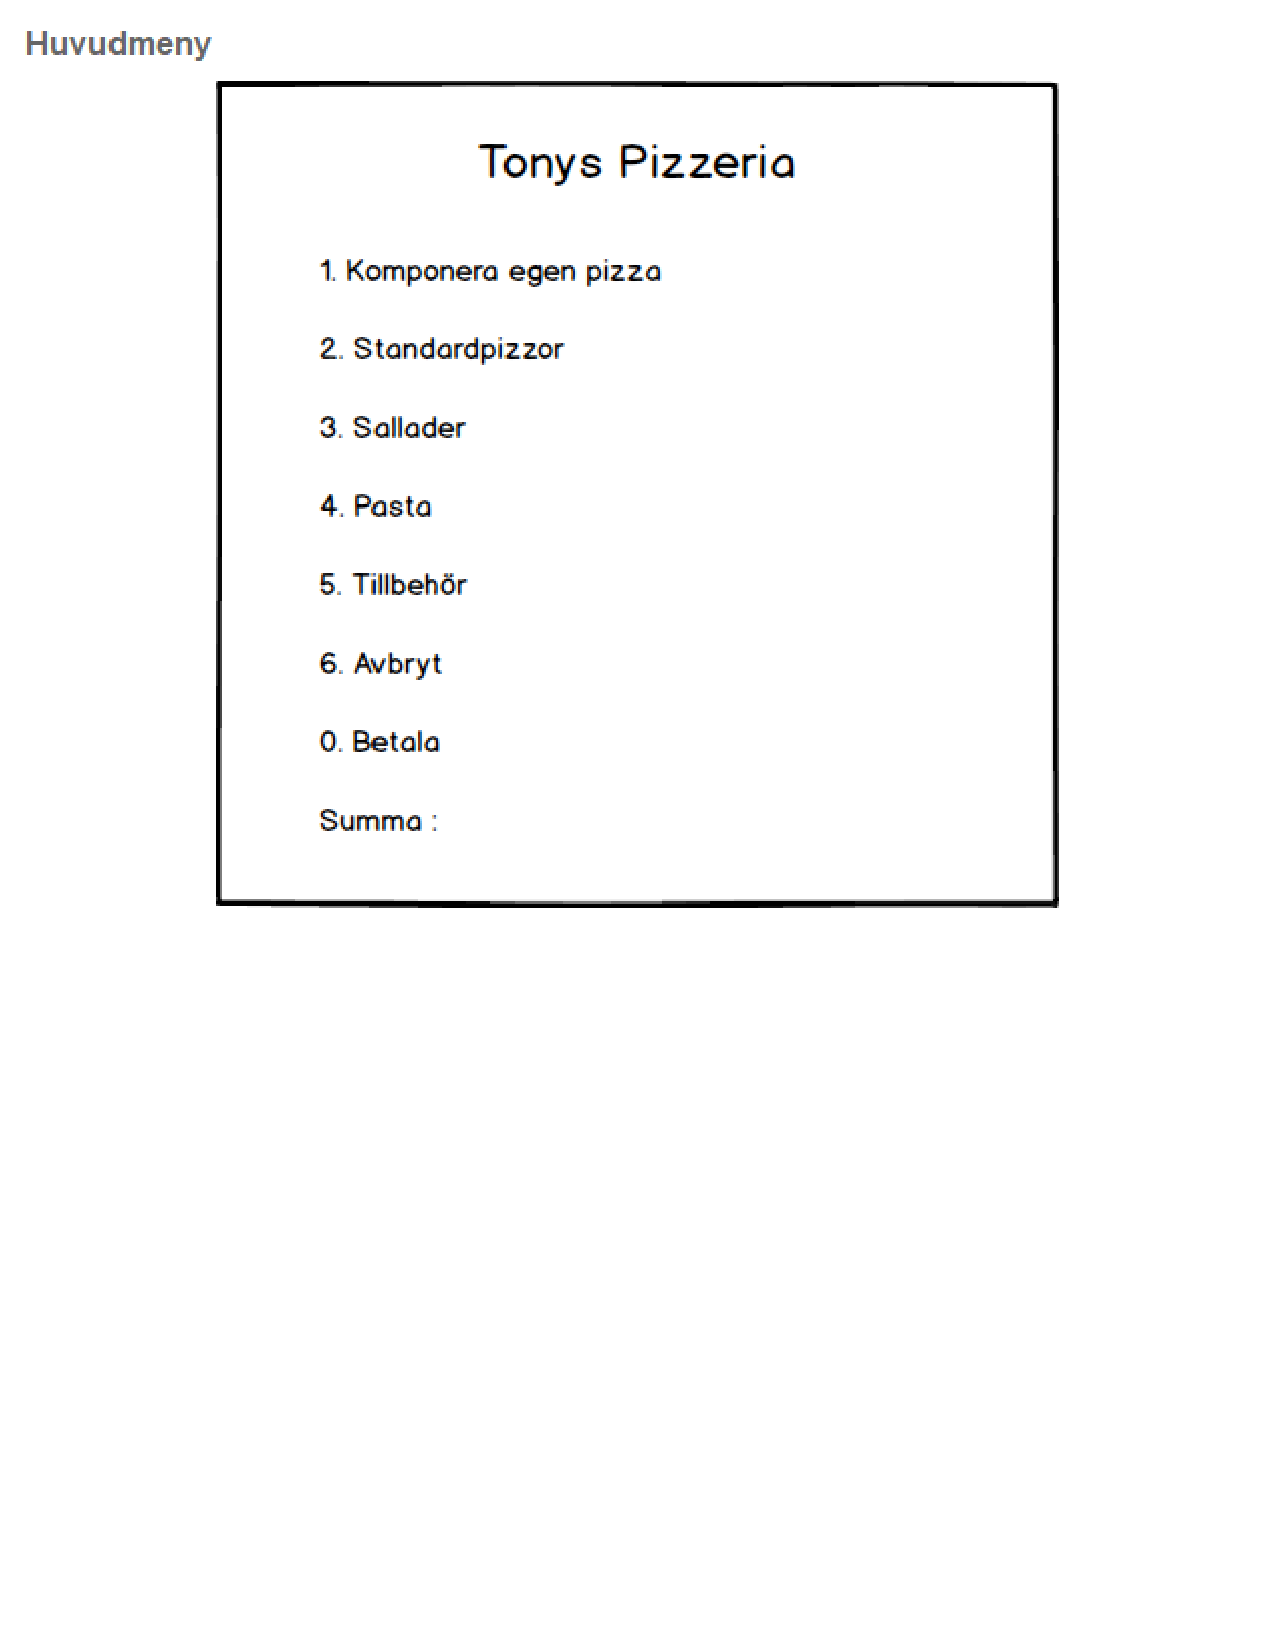
\includegraphics[width=\textwidth]{img/Skiss Tony Mozarella.pdf}
    %     \caption{BalsamIQ Skiss}
    %     %\label{fig:gull}
    % \end{subfigure}
    \index{Mockups}
    \begin{subfigure}[b]{0.3\textwidth}
        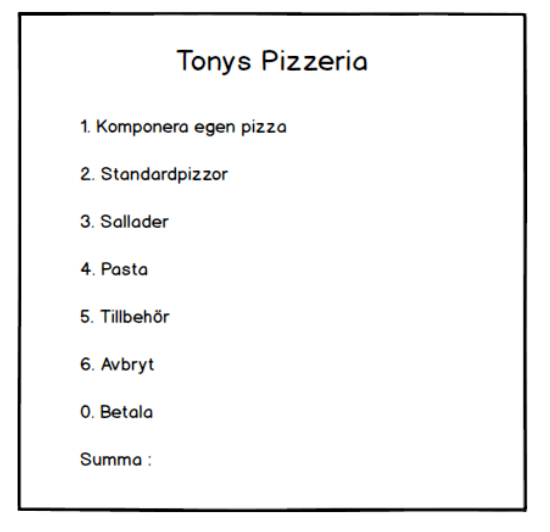
\includegraphics[width=\textwidth]{img/Skissbilder/Screen1.PNG}
        \caption{Initial kundmeny}
        %\label{fig:gull}
    \end{subfigure}
        \begin{subfigure}[b]{0.3\textwidth}
        \includegraphics[width=\textwidth]{img/Skissbilder/Screen2.PNG}
        \caption{Kvitto sida}
        %\label{fig:gull}
    \end{subfigure}
        \begin{subfigure}[b]{0.3\textwidth}
        \includegraphics[width=\textwidth]{img/Skissbilder/Screen3.PNG}
        \caption{Kundmeny}
        %\label{fig:gull}
    \end{subfigure}
        \begin{subfigure}[b]{0.3\textwidth}
        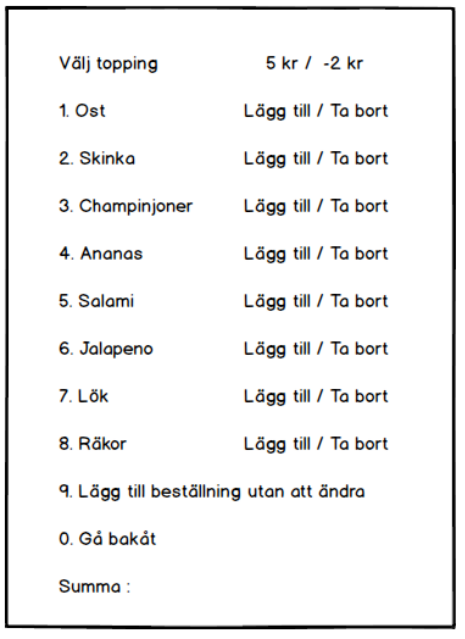
\includegraphics[width=\textwidth]{img/Skissbilder/scree6.PNG}
        \caption{Kundmeny}
        %\label{fig:gull}
    \end{subfigure}
        \begin{subfigure}[b]{0.3\textwidth}
        \includegraphics[width=\textwidth]{img/Skissbilder/Screen9.PNG}
        \caption{Del av kundmeny}
        %\label{fig:gull}
    \end{subfigure}
        \begin{subfigure}[b]{0.3\textwidth}
        \includegraphics[width=\textwidth]{img/Skissbilder/Screen10.PNG}
        \caption{Kassaterminalen}
        %\label{fig:gull}
    \end{subfigure}
        \begin{subfigure}[b]{0.7\textwidth}
        \includegraphics[width=\textwidth]{img/Skissbilder/Screen11.PNG}
        \caption{Beställningar}
        %\label{fig:Bskiss}
    \end{subfigure}
    
    
    \caption{Bilder på några av våra skisser men inte alla.}\label{fig:skisser}



\end{figure}


\subsubsection{Attityden}
En genomgripande attityd i vår grupp genom hela projektet skulle kunna vara att vår respekt för C\# ökade och att vi började nog kort sagt tycka om språket mer i takt med användningen. Något som skulle kunnat uppfattats som jobbigt var att vi oväntat skulle börja installera nya operativsystem på våra datorer i början av kursen. Vidare förväntades vi använda \index{Visual Code} \emph{Visual Code} vilket är ett relativt bra program men någorlunda överflödigt då \emph{Visual Studio} räckte gott och väl. Som förslag till framtida kurser skulle jag rekommendera att ni föreslår eleverna att installera behörighetsgivande mjukvara \emph{innan} kursen börjar eftersom dessa installationer kan göras självständigt. Förslaget är alltså att ge framtida kullar ett \emph{"förberedelse dokument"} för allt meta-arbete som kan tänkas behövas i Newtons program och kurser.

Utöver \emph{Visual Code} installerades även \index{Notepad++} \emph{notepad++} under föreläsningen improvisativt på projektor, olika \index{Linux} "linux-USB" program\footnote{Några som potentiellt innehöll \index{Malware} Malware. Mer specifikt "EaseUS Partition Master" installerades och rekommenderades explicit till eleverna.} och mer under första lektionen vi hade med läraren.
Eftersom denna kurs är första årskullen för respektive lärare kan däremot dessa oregelbundenheter tolereras. Denna repport kommer inte behandla utbildningens allmänna kvalitet genom feedback mer än så då detta är utanför rapportens syfte.

\paragraph{UML}
Innan denna sektion av rapporten avslutas kan det vara värt att tillägga ett ytterligare par ord om vår erfarenhet med "UML"-uppgifterna som ingick i  projektarbetet. \\
På föreläsningarna som vår grupp deltog aktivt i gick lärarna igenom flera punkter relaterade till UML-diagram utan att ge oss möjlighet för förberedelse till dessa. Vår grupp upplevde det dessutom som relativt frustrerande med att det inte heller fanns tydliga läsanvisningar till detta kursinnehåll. Detta noteras med tanke på vikten och resurserna som lades på ämnet från både lärare och elever. Angående källorna från nätet var det \index{UML} bekymrande för mig (och antagligen hela vår grupp) med den nästan skräckinjagande voluminösa mängd av information som fanns tillgänglig för just UML, på brist av mer objektiva uttryck om min initiala uppfattning av ämnet. Denna upplevelse dämpades inte under något sammanhang förutom då vi till synes mirakulöst fick vår UML godkänd ändå. Gruppen minns denna tid med UML som ytterst oregelbunden och kaotisk till den grad att några vägrade delta på redovisningen p.g.a frustration över situationen. När UML var färdig efter flera uppdateringar på våra roadmaps blev arbetsflödet i min mening omedelbart mer harmonisk (bortsett från de tillfällen då förslag gavs som var överkurs och därmed utanför vår implicita förkunskapsregel). För "Analys och design"-delen av denna kurs krävdes Klass- Domän och UseCasediagram varav endast vårt klassdiagram visas i Figur \ref{fig:klassdiagram}.\footnote{Domän-diagrammet och UseCase-diagrammet utelämnas från denna rapport.} \index{Diagram!Domän} \index{Diagram!UseCase}

\begin{figure}
        \index{Diagram!Klass}
        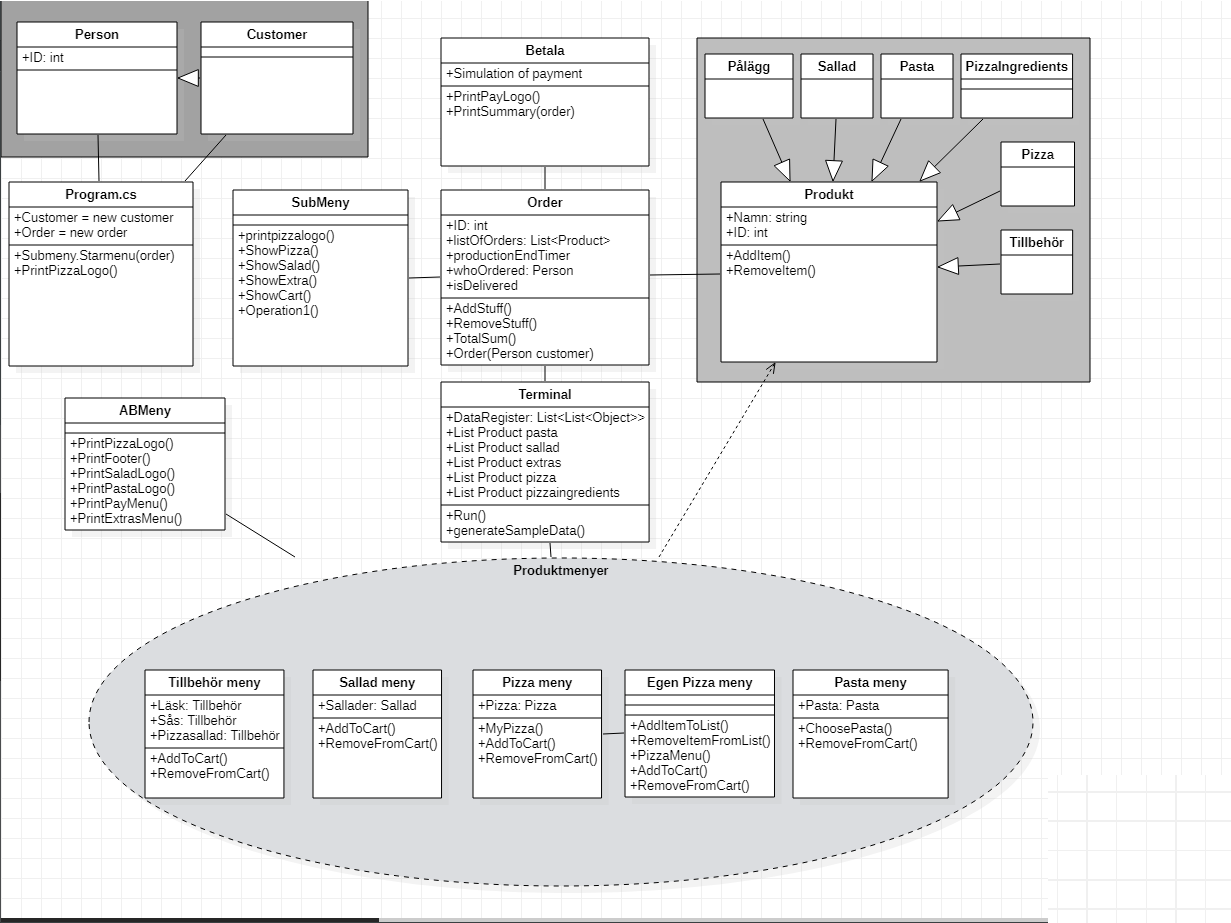
\includegraphics[width=\textwidth]{img/UML_KLASSD.PNG}
        \caption{Vårt Klass-diagram}
        \label{fig:klassdiagram}
\end{figure}

\section{Avslutningsarbetet}
Inför slutet av projektet började vi reflektera kring rapportens utformning dåd vi uppfattade att rapporten skulle lämnas in som "Gemensam Rapport". Vi uppfattade regeln om individuella rapporter som relativt överflödig då alla i gruppen kommer fram till i princip samma slutsats, nämligen att projektet var framgångsrikt och kunde levereras inom den givna tidsramen.

Mot slutet började våra kunskaper även matcha mer för varje föreläsning och kapitel som passerades i kursplanen; och detta då till allas förtjänst. Koden lades äntligen upp på \index{GIT!GitHub} GitHub\footnote{https://github.com/AdaptiveStep/PizzaPalatsetG1} 
och versionskontrollen började flöda på. När väl den sista "Roadmap 8"  publicerades hade gruppen varit i fas med både kurs och projekt. Vid skrivande stund av denna rapport återstår då endast presentation av allt samt provet till kursen (och dessutom de individuella rapporterna förstås). Vi hade vårt sista gruppmöte den 13:e november där gruppen visade hög moral och gott självförtroende inför examinerande moment. Bortsett från "UML-situationen" hade vi ett utmärkt flöde och känner oss stolta över vår insats i kursen. Uppgifterna (bortsett från UML) uppfattades som roliga och relativt lätta att koda, lite för lätta kanske. 

Terminalerna som vi framställde skilde sig dock notabelt åt i koden då vi blev färdiga med dessa. Vi upptäckte denna skillnad och fick en förståelse av hur nödvändigt det faktiskt är med användning av "Interfaces" \index{Interfaces}. Särskilt i tidiga skeden av ett grupp-projekt bör alltså interfaces designas gemensamt för att förhindra överlappande kod som uppstår vid det separata arbetet. Förbrukning av Abstrakta Klasser har vi dock inte sett en mening för i just vårt projekt. Naturligtvis inkluderade vi även en kort testfas för enklare testscenarion i det absoluta slutskedet. Dock med endast primitiva \index{Testning} "try-catch"-satser, om ens det. Vi lämnade därmed en stor del av testarbetet för nästa skeden av programmets utbildning.

\section{Sammanfattning}
Kursen började utan att ge dispens av gruppindelningen kring projektet. Det tog någon vecka innan denna gruppindelning gavs vilket gav vår grupp ett intryck om godtycklighet. Jämfört med andra grupper i klassen låg kanske vår grupp bäst till gällande projektets framfart (och kanske till och med inspirerade andra gruppers arbete). Vår grupp (Grupp1) har undersökt, utrett, utvecklat och diskuterat med både lärare och varandra kring olika aspekter i allt från nuvarande kurs till framtida implementationer av givna uppgifter. 

% UML-delen i kursen saknade i allmänhet lämpliga anvisningar till litteratur och orsakade disproportionell frustration för vår grupp. \kommentar{kanske onödig sista avslutande mening. Ty för mycket irriterande feedback.}

Från denna rapport kan det som tidigare nämndes rekommenderas att framtida kullar har UML-delen endast i senare kurser av programmet. Arbetsbördan var låg vid kodningen, utbildningsledarna följde upp med utbildningen och var aktiva med att ge stöd, idéer och tips. Några av våra medlemmar deltog mer eller mindre än andra men i slutändan lyckades gruppen med god marginal leverera önskvärt resultat. 

Tack. 
\vspace*{1cm \hfill /H}

\clearpage

%%%%%%%%%%%%%%%%%%%%%%%%%%%%%%%%%%%%%%%%%%%%
%%%%%%  Rör ej nedanstående             %%%%
%%%%%%   Ändra endast om                %%%%
%%%%%%   du vill ta bort                %%%%
%%%%%%   hela referens sidan.           %%%%
%%%%%% Kommentera då ut dessa tre rader %%%%
%\newpage                               %%%% %-Kommentera ut
%\bibliographystyle{siam}               %%%% %-Kommentera ut
%\bibliography{references.bib}          %%%% %-Kommentera ut
%%%%%%%%%%%%%%%%%%%%%%%%%%%%%%%%%%%%%%%%%%%%
%%%%%%%%%%%%%%%%%%%%%%%%%%%%%%%%%%%%%%%%%%%%

\printindex

\end{document}

% Hoppas det går bra!
% Lycka till med uppsatsen!